% this is a template for papers or notes written in Chinese
\documentclass[a4paper]{report}
\usepackage{mdframed}
\usepackage{hyperref}
\usepackage{booktabs}
\usepackage{makecell}
\usepackage{longtable}
\usepackage{xeCJK}
\usepackage{titletoc}
\usepackage{ulem}
\usepackage{stringstrings}
\usepackage{zhnumber}
\makeatletter
\newcommand{\mytitle}{\@title}
\makeatother

\usepackage[
    fontset=none,%设置中文支持,并自定义字体
    zihao=5,%默认字号为五号
    heading=true,%允许后续自定义标题样式
    scheme=chinese,%自动将文档样式中文化,例如图标标题
    punct=quanjiao,%全角式标点符号
    space=auto,%中文后接换行不会添加空格,但是英文会添加空格,需要用%手动取消
    % linespread=1.3,%行距倍数是1.3
    autoindent=true,%自动缩进两个中文宽度
    ]{ctex}

\ctexset{
    today=small,%小写样式的日期
    contentsname={目录},
    % contentsname={\hspace{-\ccwd}目录},
    listfigurename={插图},
    listtablename={表格},
    figurename={图},
    tablename={表},
    abstractname={简{\quad}介},
    indexname={索引},
    appendixname={附录},
    bibname={参考文献},
    proofname={证明},
    % refname={参考文献},%只适用于beamer
    % algorithmname={算法},
    % continuation={(续)},%beamer续页的标识
    chapter={
        format+ = \Huge\heiti\raggedright,
        name = {,\num\textbf{.}\hspace{1ex}},
        number={\num\thechapter},
        nameformat={},
        numberformat={},
        aftername={},
        titleformat={},
        aftertitle={},
        runin=false,%对section级以下有用,标题是否和正文在同一段上
        beforeskip={3.5ex plus 1ex minus .2ex},%标题前垂直间距
        afterskip={2.3ex plus .2ex}%标题后垂直间距
    },
    section={
        format+ = \Large\heiti\raggedright,
        name = {,\num\textbf{.}\hspace{1ex}},
        number={\num\thesection},
        nameformat={},
        numberformat={},
        aftername={},
        titleformat={},
        aftertitle={},
        runin=false,%对section级以下有用,标题是否和正文在同一段上
        beforeskip={3.5ex plus 1ex minus .2ex},%标题前垂直间距
        afterskip={2.3ex plus .2ex}%标题后垂直间距
    },
    subsection={
        format+ = \large\heiti\raggedright,
        name = {,\num\textbf{.}\hspace{1ex}},
        number={\num\thesubsection},
        nameformat={},
        numberformat={},
        aftername={},
        titleformat={},
        aftertitle={},
        runin=false,%对section级以下有用,标题是否和正文在同一段上
        beforeskip={3.5ex plus 1ex minus .2ex},%标题前垂直间距
        afterskip={2.3ex plus .2ex}%标题后垂直间距
    },
    subsubsection={
        format+ = \normalsize\heiti\raggedright,
        name = {,\num\textbf{.}\hspace{1ex}},
        number={\num\thesubsubsection},
        nameformat={},
        numberformat={},
        aftername={},
        titleformat={},
        aftertitle={},
        runin=false,%对section级以下有用,标题是否和正文在同一段上
        beforeskip={3.5ex plus 1ex minus .2ex},%标题前垂直间距
        afterskip={2.3ex plus .2ex}%标题后垂直间距
    },
    }

\usepackage{amsfonts}
\usepackage{lmodern}%解决报错
% 中文默认字体: 思源宋体,粗体为思源宋体半粗体,斜体为方正楷体_GBK
\setCJKmainfont{Source Han Serif SC}[BoldFont={Source Han Serif SC Heavy}, ItalicFont=FZKai-Z03S]
% 中文无衬线字体:思源黑体,粗体为思源黑体粗体
\setCJKsansfont{Source Han Sans CN}[BoldFont={Source Han Sans CN Heavy}]
% 中文等宽字体:微软雅黑light
\setCJKmonofont{Microsoft YaHei}[ItalicFont={Microsoft YaHei Light}]

\newCJKfontfamily\songti{Source Han Serif SC}[BoldFont={Source Han Serif SC Heavy}]
\newCJKfontfamily\xbsong{Source Han Serif SC SemiBold} % 小标宋
\newCJKfontfamily\dbsong{Source Han Serif SC Bold} % 大标宋
\newCJKfontfamily\cusong{Source Han Serif SC Heavy} % 粗宋
\newCJKfontfamily\heiti{Source Han Sans CN}[BoldFont={Source Han Sans CN Heavy}]
\newCJKfontfamily\dahei{Source Han Sans CN Medium} % 大黑
\newCJKfontfamily\cuhei{Source Han Sans CN Heavy} % 粗黑
\newCJKfontfamily\fangsong{FZFangSong-Z02S}
\newCJKfontfamily\kaiti{FZKai-Z03S}[ItalicFont={Microsoft YaHei Light}]%这个斜体只是用于lstlisting环境中的中文注释
% \newCJKfontfamily\kaiti{FZKai-Z03S}[ItalicFont={FZZJ-LZXTFSJW}]%这个斜体只是用于lstlisting环境中的中文注释
\setsansfont{Arial}
\setmonofont{Consolas}%设置西文等宽字体
\newfontfamily\code{Consolas}
\newfontfamily\num{Arial}

\usepackage{geometry}%设置整体页面布局
\geometry{a4paper}
\geometry{left=2cm,right=2cm,top=2.54cm,bottom=2.54cm}%word常规页边距
% \geometry{left=1.27cm,right=1.27cm,top=1.27cm,bottom=1.27cm}%word窄页边距
\setlength{\headheight}{13pt}%避免warning


\usepackage{fancyhdr}%必须在geometry包之后使用
\fancyhf{}
\lhead{\sffamily\bfseries{范潇 2254298}}%可以使用thepage,CTEXthechapter,CTEXthesection
\chead{\sffamily\bfseries{课程设计作业Project5}}
\rhead{\sffamily\bfseries{- \thepage{} -}}
\renewcommand\headrulewidth{2pt}%设置眉头宽度
\pagestyle{fancy}


\usepackage{tikz}
\usepackage{graphicx}
\usepackage{longtable}
\usepackage{amssymb}
\newcommand*{\abs}[1]{\lvert #1 \rvert}
\setlength{\baselineskip}{18pt}
\usepackage{float}
\usepackage[ruled,algosection,lined,longend,fillcomment,linesnumbered,resetcount,titlenotnumbered]{algorithm2e}
%参数解释:带框,按section编码,有竖线,end前带if等关键词,注释占满整行,代码部分编号(不包括输入输出、注释),每个代码块重新编号,可以调用TitleOfAlgo来打印算法标题但不作为单独的算法编码
%附带algorithm,function,procedure环境,其中function,procedure环境下,设置caption时,必须带有(),
%()之前的字符会被视为宏,可以在接下来的部分用\名字()来调用,所以推荐辅助函数用function,其中的某些展开部分用procedure,描述算法整体使用algorithm
\DontPrintSemicolon
\SetAlCapSkip{2ex}
\SetSideCommentRight
\SetFillComment
\newcommand{\forcond}{$i=0$ \KwTo $n$}
\SetKw{macro}{text}%自定义关键词
\SetKwFunction{funcmacro}{text}%自定义函数名,实际上function环境是在定义宏的同时说明了其内容
\SetKwProg{procedmacro}{text}{begin text}{end text}%自定义步骤,和function类似,但是后面两个参数可以设置开始和结尾的标志,和if等环境一样
\SetKwData{datamacro}{text}%可以用于突出特殊的变量,例如数据结构
\SetKwFunction{FRecurs}{FnRecursive}
\SetKwProg{Fn}{Function}{begin}{end}
\usepackage{xcolor}%颜色支持
\definecolor{vscode_backgroundcolor}{rgb}{0.15, 0.2, 0.22}
\definecolor{vscode_localvariablecolor}{rgb}{0.93,1,0.89}
\definecolor{vscode_keywordcolor}{rgb}{0.57, 0.52, 1}
\definecolor{vscode_commentcolor}{rgb}{0.2, 0.34, 0.45}
\definecolor{vscode_stringcolor}{rgb}{0.76, 0.91, 0.55}
\definecolor{vscode_semicolomncolor}{rgb}{1,1,1}
\definecolor{vscode_headerfilecolor}{rgb}{0.93,1,0.89}
\definecolor{vscode_linenumbercolor}{rgb}{0.2, 0.34, 0.45}
\definecolor{vscode_numbercolor}{rgb}{0.96, 0.54, 0.42}
\definecolor{vscode_parametercolor}{rgb}{0.96, 0.54, 0.42}
\definecolor{vscode_operatorcolor}{rgb}{0.53, 0.85, 0.99}
\definecolor{vscode_callablecolor}{rgb}{0.36, 0.62, 0.96}
\definecolor{vscode_rulecolor}{rgb}{0.22, 0.28, 0.31}
\definecolor{vscode_classcolor}{rgb}{1, 0.8, 0.42}
\definecolor{vscode_selfcolor}{rgb}{0.97, 0.31, 0.43}

\usepackage{listings}%高亮代码块支持
\lstloadlanguages{Python}
\lstdefinestyle{MyPython}{
    extendedchars=false,
    numbers=left,
    firstnumber=auto,
    frame=leftline,
    backgroundcolor=\color{vscode_backgroundcolor},
    framerule=0.5ex,
    columns=fixed,
    language=Python,
    basicstyle=\ttfamily\color{vscode_localvariablecolor},
    % commentstyle=\color{vscode_commentcolor},
    keywordstyle=\color{vscode_keywordcolor},
    stringstyle=\color{vscode_stringcolor},
    morecomment=[l][\color{vscode_commentcolor}]{\#},
    morecomment=[s][\color{vscode_headerfilecolor}]{"""}{"""},
    numberstyle=\code\color{vscode_linenumbercolor},
    morekeywords={
        None,
        True,
        yield,
        False,
    },
    alsoletter={
        =+-*<>^&
        % ;0123456789
        % 0,1,2,3,4,5,6,7,8,9
    },%把;设置为可以识别的letter,也可以使用otherkeywords,但是无法将其和其他keywords区分开来
    emph={=,+,-,*,>,<,<<,>>,^,+=,&},emphstyle=\color{vscode_operatorcolor},
    % alsoletter={!,\%,&,*,-,+,=,/,<,>},
    emph={[2]%一些全局的函数和可调用对象
    namedtuple,
    list2tuple,
    list,
    tuple, 
    generalGraphSearch,
    float,
    isinstance,
    Property,
    PriorityQueue,
    getSuccessors,
    getStartState,
    isGoalState,
    push,
    pop,
    isEmpty,
    get_solution,
    keys,
    cnt,
    next,
    dfsPriority,
    bfsPriority,
    ucsPriority,
    AStarPriority,
    append,
    aStarSearch,
    depthFirstSearch,
    breadthFirstSearch,
    uniformCostSearch,
    len,
    index,
    Successors,
    int,
    directionToVector,
    greedy,
    manhattanDistance,
    remove,
    cornersHeuristic,
    enumerate,
    foodHeuristic,
    max,
    range,
    asList,
    findPathToClosestDot,
    getPacmanPosition,
    getFood,
    getWalls,
    AnyFoodSearchProblem,
    evaluationFunction,
    generatePacmanSuccessor,
    getGhostStates,
    float,
    len,
    maximize,
    minimize,
    getLegalActions,
    evaluationFunction,
    generateSuccessor,
    getNumAgents,
    randomMove,
    run,
    train,
    get,
    prediction,
    iterate,
    once,
    as,
    scalar,
    DotProduct,
    update,
    Parameter,
    AddBias,
    Linear,
    ReLU,
    SquareLoss,
    gradients,
    init,
    mid,
    log,
    SoftmaxLoss
    },emphstyle={[2]\color{vscode_callablecolor}},
    emph={[5]
    self},emphstyle={[5]\color{vscode_selfcolor}},
    % emphstyle={[3]\color{vscode_parametercolor}}
     % emph={[3]0,1,2,3,4,5,6,7,8,9},emphstyle={[3]\color{yellow}},
    tabsize=4,
    rulecolor=\color{vscode_rulecolor},
    breaklines=true,
}
\lstset{
    style=MyPython,
}
% \usepackage{xcolor}%颜色支持
\definecolor{vscode_backgroundcolor}{rgb}{0,0.14,0.32}
\definecolor{vscode_localvariablecolor}{rgb}{0.94,0.62,0.64}
\definecolor{vscode_keywordcolor}{rgb}{0.92,0.73,1}
\definecolor{vscode_commentcolor}{rgb}{0.55,0.64,0.79}
\definecolor{vscode_stringcolor}{rgb}{0.05,0.95,0.86}
\definecolor{vscode_semicolomncolor}{rgb}{1,1,1}
\definecolor{vscode_headerfilecolor}{rgb}{0.82,0.95,0.65}
\definecolor{vscode_linenumbercolor}{rgb}{0.52,0.52,0.52}
\definecolor{vscode_numbercolor}{rgb}{1,0.77.0.56}
\definecolor{vscode_operatorcolor}{rgb}{0.6,1,1}
\definecolor{vscode_functioncolor}{rgb}{0.22,0.65,0.96}
\definecolor{vscode_rulecolor}{rgb}{0.17,0.46,0.65}

\usepackage{amsmath}%必须在amsthm之前
\usepackage{amsthm}%提供证明,定理等环境

\theoremstyle{plain}
\newtheorem{thm}{Theorem}[section]
\newtheorem{lmm}{Lemma}[section]
\newtheorem{cor}{Corollary}[section]
\newtheorem{prop}{Proposition}[section]
\newtheorem{conj}{Conjecture}[section]

\theoremstyle{definition}
\newtheorem{definition}{Definition}[section]
\newtheorem*{cond}{Condition}
\newtheorem{eg}{Example}[section]
\newtheorem{exer}{Exercise}[section]
\newtheorem*{property}{Property}

\theoremstyle{remark}
\newtheorem*{rmk}{Remark}


\usepackage[strict]{changepage}
\usepackage{framed}%色块支持
\definecolor{formalshade}{rgb}{0.95,0.95,1} % 文本框颜色
% ------------------******-------------------
% 注意行末需要把空格注释掉,不然画出来的方框会有空白竖线

\definecolor{theorem_bar_color}{RGB}{183, 28, 28}
\definecolor{theorem_box_color}{RGB}{255, 235, 238}
\newenvironment{mythm}[1][]{%
\def\FrameCommand{%
\hspace{1pt}%
{\color{theorem_bar_color}\vrule width 2pt}%
{\color{theorem_box_color}\vrule width 4pt}%
\colorbox{theorem_box_color}%
}%
\MakeFramed{\advance\hsize-\width\FrameRestore}%
\noindent\hspace{-4.55pt}% disable indenting first paragraph
\begin{adjustwidth}{}{7pt}%
\begin{thm}[#1]
    \quad\par
}
{%
\end{thm}
\vspace{2pt}\end{adjustwidth}\endMakeFramed%
}

\definecolor{corollary_bar_color}{RGB}{26, 35, 126}
\definecolor{corollary_box_color}{RGB}{232, 234, 246}
\newenvironment{mycor}[1][]{%
\def\FrameCommand{%
\hspace{1pt}%
{\color{corollary_bar_color}\vrule width 2pt}%
{\color{corollary_box_color}\vrule width 4pt}%
\colorbox{corollary_box_color}%
}%
\MakeFramed{\advance\hsize-\width\FrameRestore}%
\noindent\hspace{-4.55pt}% disable indenting first paragraph
\begin{adjustwidth}{}{7pt}%
\begin{cor}[#1]
    \quad\par
}
{%
\end{cor}
\vspace{2pt}\end{adjustwidth}\endMakeFramed%
}

\definecolor{lemma_bar_color}{RGB}{74, 20, 140}
\definecolor{lemma_box_color}{RGB}{243, 229, 245}
\newenvironment{mylmm}[1][]{%
\def\FrameCommand{%
\hspace{1pt}%
{\color{lemma_bar_color}\vrule width 2pt}%
{\color{lemma_box_color}\vrule width 4pt}%
\colorbox{lemma_box_color}%
}%
\MakeFramed{\advance\hsize-\width\FrameRestore}%
\noindent\hspace{-4.55pt}% disable indenting first paragraph
\begin{adjustwidth}{}{7pt}%
\begin{lmm}[#1]
    \quad\par
}
{%
\end{lmm}
\vspace{2pt}\end{adjustwidth}\endMakeFramed%
}

\definecolor{proposition_bar_color}{RGB}{1, 87, 155}
\definecolor{proposition_box_color}{RGB}{225, 245, 254}
\newenvironment{myprop}[1][]{%
\def\FrameCommand{%
\hspace{1pt}%
{\color{proposition_bar_color}\vrule width 2pt}%
{\color{proposition_box_color}\vrule width 4pt}%
\colorbox{proposition_box_color}%
}%
\MakeFramed{\advance\hsize-\width\FrameRestore}%
\noindent\hspace{-4.55pt}% disable indenting first paragraph
\begin{adjustwidth}{}{7pt}%
\begin{prop}[#1]
    \quad\par
}
{%
\end{prop}
\vspace{2pt}\end{adjustwidth}\endMakeFramed%
}

\definecolor{definition_bar_color}{RGB}{0, 77, 64}
\definecolor{definition_box_color}{RGB}{224, 242, 241}
\newenvironment{mydef}[1][]{%
\def\FrameCommand{%
\hspace{1pt}%
{\color{definition_bar_color}\vrule width 2pt}%
{\color{definition_box_color}\vrule width 4pt}%
\colorbox{definition_box_color}%
}%
\MakeFramed{\advance\hsize-\width\FrameRestore}%
\noindent\hspace{-4.55pt}% disable indenting first paragraph
\begin{adjustwidth}{}{7pt}%
\begin{definition}[#1]
    \quad\par
}
{%
\end{definition}
\vspace{2pt}\end{adjustwidth}\endMakeFramed%
}

\definecolor{remark_bar_color}{RGB}{245, 127, 23}
\definecolor{remark_box_color}{RGB}{255, 253, 231}
\newenvironment{myrmk}[1][]{%
\def\FrameCommand{%
\hspace{1pt}%
{\color{remark_bar_color}\vrule width 2pt}%
{\color{remark_box_color}\vrule width 4pt}%
\colorbox{remark_box_color}%
}%
\MakeFramed{\advance\hsize-\width\FrameRestore}%
\noindent\hspace{-4.55pt}% disable indenting first paragraph
\begin{adjustwidth}{}{7pt}%
\begin{rmk}[#1]
    \quad\par
}
{%
\end{rmk}
\vspace{2pt}\end{adjustwidth}\endMakeFramed%
}

\definecolor{property_bar_color}{RGB}{62, 39, 35}
\definecolor{property_box_color}{RGB}{239, 235, 233}
\newenvironment{myproperty}[1][]{%
\def\FrameCommand{%
\hspace{1pt}%
{\color{property_bar_color}\vrule width 2pt}%
{\color{property_box_color}\vrule width 4pt}%
\colorbox{property_box_color}%
}%
\MakeFramed{\advance\hsize-\width\FrameRestore}%
\noindent\hspace{-4.55pt}% disable indenting first paragraph
\begin{adjustwidth}{}{7pt}%
\begin{property}[#1]
    \quad\par
}
{%
\end{property}
\vspace{2pt}\end{adjustwidth}\endMakeFramed%
}

\author{\Large{范潇\quad2254298}}
\title{\sffamily\Huge\bfseries{数据库课程设计报告}}
\date{\Large{\today}}
\pagestyle{empty}
\renewcommand{\contentsname}{\textcolor[rgb]{0.54,0.62,0.83}{\textnormal{\fontsize{16pt}{0}{目录}}}}
\titlecontents{chapter}
[0pt]
{\vspace{0pt}\zihao{5}}              
{\thecontentslabel}              
{}
{\titlerule*[8pt]{.}\contentspage}

\begin{document}
\begin{titlepage}
    \heiti
    \vspace*{64pt}
    \begin{center}
        \fontsize{24pt}{0}{城市共享单车管理与调度系统}\\
        \vspace*{36pt}
        \fontsize{16pt}{0}{数据库原理课程设计报告}\\
        \vspace*{50pt}
        
\includegraphics{./pic/tongji-logo-purple.pdf}\\
        \vspace*{50pt}
        \fontsize{14pt}{0}{学  号}\ \ \underline{\makebox[200pt]{\fontsize{14pt}{0}{\songti\textbf{2254298}}}}\\
        \vspace*{10pt}
        \fontsize{14pt}{0}{姓  名}\ \ \underline{\makebox[200pt]{\fontsize{14pt}{0}{\songti\textbf{范潇}}}}\\
        \vspace*{10pt}
        \fontsize{14pt}{0}{专  业}\ \ \underline{\makebox[200pt]{\fontsize{14pt}{0}{\songti\textbf{数据科学与大数据技术}}}}\\
        \vspace*{10pt}
        \fontsize{14pt}{0}{授课老师}\ \ \underline{\makebox[200pt]{\fontsize{14pt}{0}{\songti\textbf{李文根}}}}\\
        \vspace*{36pt}
    \end{center}
\end{titlepage}
\tableofcontents
\noindent\fontsize{12pt}{0}{\fangsong\textbf{摘\quad 要}}
\addcontentsline{toc}{chapter}{城市共享单车管理与调度系统} 
{\fangsong
近年来,共享单车作为“最后一公里”的解决方案得到了广泛的推广,市场中涌现出大量共享单车公司。在整个运营过程中由智能
技术提供支持,企业负责整个运营过程中的管理。消费者在选择共享单车品牌时,除了定价、押金等经济因素,还会着重考量单车性能、维护质量和单车分布等体验因素。
同时,由于共享单车市场的快速发展,交通运输部等10部门也对共享单车(互联网租凭自行车)行业发布指导意见,要求“引导有序投放车辆”、“加强互联网租凭自行车标准化建设”、“加强停放管理和监督执法”,“引导用户安全文明用车”等。

综上,共享单车管理与调度系统无论对于共享单车企业提升市场竞争力,还是满足行业指导意见,都至关重要。
因此,在本项目中,我为一个假想的小型共享单车公司开发共享单车管理与调度系统。该系统采用基于角色的鉴权系统。
单车和调度人员可以通过系统开放的API接口上传数据;分析团队人员可以通过平台生成查看单车分布图、生成调度日志、生成单车使用情况的空间分布和生成单车状况统计信息;
管理人员在分析团队人员的权限基础之上,还可以通过平台添加或删除单车或停车区域信息。同时还可以通过平台全局更新共享单车的状态。




本项目在概念设计过程中构建了以下实体集:
   \textit{bike(\underline{bike\_ID},production\_date,coordinate,\\status,battery\_remaining\_capacity)};
   \textit{usage(\dotuline{time},coordinate,action)};
   \textit{parking\_area(\underline{parking\_area\_ID},\\name,coordinate,radius)};
   \textit{scheduling(\dotuline{time},coordinate,action)};
   \textit{to\_be\_reviewed(\dotuline{time},status,proof\_material)};


本项目在概念设计过程中构建了以下关系集:
   \textit{bike\_usage}:将单车和单车使用记录关联在一起;
   \textit{contain}:将单车和单车停车区域关联在一起;
   \textit{bike\_scheduling}:将单车和单车调度记录关联在一起;
   \textit{bike\_to\_be\_reviewed}:将单车和待审查记录关联在一起;

上述实体集和关系集在逻辑设计过程中被转变为了实体集模式和关系集模式,均满足BC范式。

本系统
使用Next.js进行全栈开发。
对于前端,我使用Next.js,React和NextUI来构建页面和组件。使用Tailwind CSS进行样式设计。
同时,我使用Next.js了最新推出的文件系统路由,将文件自动映射到网页或网页布局;
对于后端,绝大部分的功能,如用户认证、表单提交和数据处理,我都通过Next.js提供的Server Actions功能来实现。
对于调度员和单车上传数据的需求,我仍然通过API路由来
接受他们所上传的信息,但是后续的处理仍然是通过Server Actions来实现。在数据管理部分,我通过Drizzle ORM
与Postgres数据库进行交互,并且通过数据访问层(DAL)来保障数据安全。

本次实验报告为最终报告设计,包含需求分析、可行性分析、概念设计、逻辑设计、项目管理、项目实现以及总结。
}

\noindent\fontsize{12pt}{0}{\textbf{关键词:共享单车、管理、调度、数据库、Postgres、Next.js}}
\chapter{概述}
\thispagestyle{empty}
\section{课题背景}
共享单车作为共享经济的新形态,
是指企业与政府进行合作,在居民区、商业区、地铁站、公交车
站、校园等公共场所提供自行车骑行的共享服务。它是借助互
联网技术推出的一种分时租赁业务。在整个运营过程中由智能
技术提供支持,企业负责整个运营过程中的管理\cite{article1}。

消费者在选择共享单车品牌时,除了定价、押金等经济因素,还会着重考量以下体验因素:
\begin{itemize}
    \item 单车性能:例如单车重量,可调节性等;
    \item 维护质量:是否有大量未及时回收的损坏单车;
    \item 单车分布:单车的时空分布是否符合使用需求的时空分布。
\end{itemize}

同时,由于共享单车市场的快速发展,交通运输部等10部门也对共享单车(互联网租凭自行车)行业发布指导意见,要求“引导有序投放车辆”、“加强互联网租凭自行车标准化建设”、“加强停放管理和监督执法”,“引导用户安全文明用车”等。

\section{编写目的}

本课题旨在为一个虚构的新创共享单车公司开发单车管理与调度平台,以帮助公司的工作人员对该公司的共享单车进行管理与调度,达到提升公司市场竞争力、符合政府规范的最终目的。

结合当今各大共享单车公司,如美团单车、哈喽单车等,的运营模式,我们对于该公司作以下假设:
\begin{enumerate}
    \item 出于存储代价的考量,该公司的数据库中不保存历史数据。例如,对于“单车”实体,只保存其最近上传的坐标;
    \item 该公司使用的共享单车只会在开关锁的时候向系统上传信息;
    \item 运维人员的运维任务由组长通过微信、钉钉等工具下发,或者自行根据实际情况实施调度(因此不在数据库中进行记录);
    \item 要求用户将车辆停放在指定停车区域内(因此需要对于停车区域进行建模)。
\end{enumerate}

由于本次设计的平台用于共享单车企业的共享单车管理与调度。因此,所用数据库中存储的数据均围绕“共享单车”这一主体,
并不涉及共享单车用户的余额、购买的月卡套餐等信息,从而并未对共享单车用户进行建模。


\chapter{需求分析}\label{chap:feasibility}
\thispagestyle{empty}
\section{功能需求}
% 本平台的用户可以分为三类:分析团队、调度员和管理者。

对于分析团队,他们对该平台有以下需求:
\begin{enumerate}
    \item 由平台生成查看单车分布图,对应图\ref{GenerateBikeDistributionMap}中的用例\texttt{Generate Bike Distribution Map};
    \item 由平台生成调度日志,对应图\ref{ProduceBikeSchedulingLog}中的用例\texttt{Produce Bike Scheduling Log};
    \item 由平台生成单车使用情况的空间分布,对应图\ref{GenerateBikeUsageMap}中的用例\texttt{Generate Bike Usage Map}。
    \item 由平台生成单车状况统计信息,对应图\ref{ProduceBikeStatusStatistics}中的用例\texttt{Produce Bike Status Statistics}。
\end{enumerate}

对于调度员,他们对于该平台有以下需求:
\begin{enumerate}
    \item 调度员可以在平台中上传调度信息,对应图\ref{UploadSchedulingLog}中的用例\texttt{Upload Scheduling Log};
    \item 调度员可以在平台中更新单车状态信息,对应图\ref{UpdateSingleBikeStatus}中的用例\texttt{Update Single Bike Status}。
\end{enumerate}

对于管理者,在分析团队的需求基础之上,他们对于该平台有还以下需求:
\begin{enumerate}
    \item 管理者可以通过平台添加或删除单车信息,对应图\ref{ModifyBikeList}中的用例\texttt{Modify Bike List};
    \item 管理者可以通过平台添加或删除停车区域信息,对应图\ref{ModifyParkingAreaList}中的用例\texttt{Modify Parking Area List}。
    \item 通过平台全局更新单车状态,对应图\ref{UpdateBikeStatusGlobally}中的用例\texttt{Update Bike Status Globally}。
\end{enumerate}

处于安全性考虑,平台还需要对上述三类用户进行分级。

同时,该平台需要处理由共享单车在开关锁时上传的信息,对应图\ref{UpdateBikeInformation}中的用例\texttt{Update Bike Info}。

整个系统的用例汇总如图\ref{UseCase}所示。

\begin{figure}[!htbp]
    \centering
    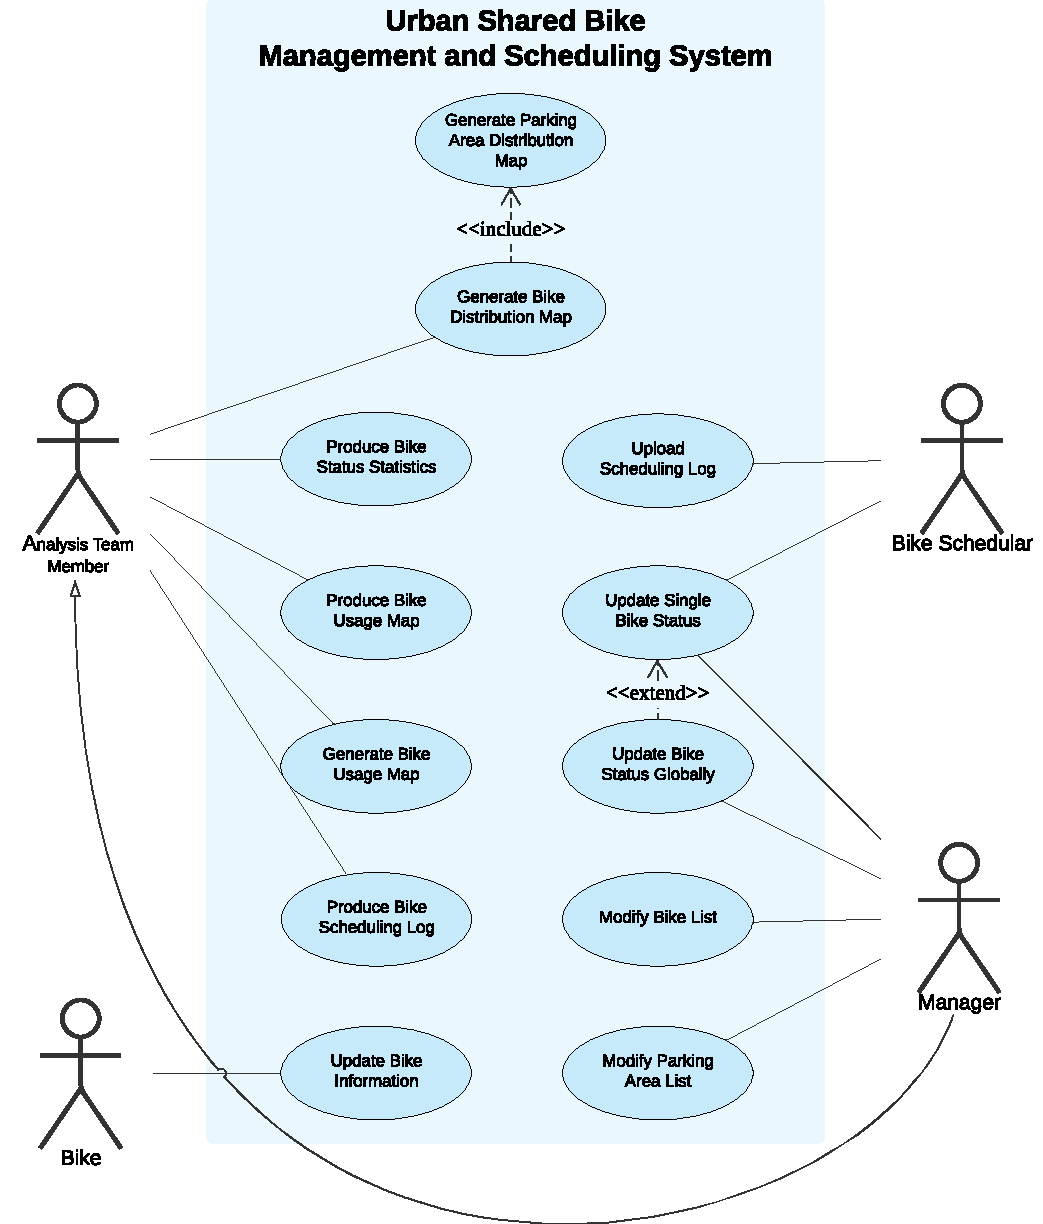
\includegraphics[width=0.99\textwidth]{figures/UseCase.pdf}
    \caption{用例汇总}\label{UseCase}
\end{figure}


\begin{figure}
    \centering
 \begin{mdframed}[leftmargin=0pt, rightmargin=0pt]
    \textbf{简要说明}

    用例\texttt{Generate Bike Distribution Map}使得分析团队成员和调度员能够查看共享单车的实时分布。

\noindent\rule{\textwidth}{0.5pt} % 实线分割线
    \textbf{分步说明}

    \begin{enumerate}
        \item 系统从数据库中收集所有共享单车的坐标及其状态;
        \item 系统依据单车坐标将单车标注在电子地图中;
        \item 系统依据单车坐标生成热力图;
        \item 系统通过用例\texttt{Generate Parking Area Distribution Map}在地图中标注停车区域;
        \item 系统调整地图窗口显示区域。
    \end{enumerate}
\end{mdframed}   
\caption{用例\texttt{Generate Bike Distribution Map}}\label{GenerateBikeDistributionMap}
\end{figure}

\begin{figure}
    \centering
 \begin{mdframed}[leftmargin=0pt, rightmargin=0pt]
    \textbf{简要说明}

    用例\texttt{Generate Parking Area Distribution Map}使得分析团队成员和调度员能够查看停车区域的分布情况。

\noindent\rule{\textwidth}{0.5pt} % 实线分割线
    \textbf{分步说明}

    \begin{enumerate}
        \item 系统从数据库中收集所有停车区域的中心坐标与半径;
        \item 系统利用中心坐标与半径在地图中绘制圆形区域以表示停车区域;
    \end{enumerate}
\end{mdframed}   
\caption{用例\texttt{Generate Parking Area Distribution Map}}\label{GenerateParkingAreaDistributionMap}
\end{figure}

\begin{figure}
    \centering
 \begin{mdframed}[leftmargin=0pt, rightmargin=0pt]
    \textbf{简要说明}

    用例\texttt{Upload Scheduling Log}使得调度员能够上传调度日志。

\noindent\rule{\textwidth}{0.5pt} % 实线分割线
    \textbf{分步说明}

    \begin{enumerate}
        \item 调度员通过API接口向系统上传调度日志;
        \item 系统将数据保存至\texttt{scheduling}表中;
    \end{enumerate}
\end{mdframed}   
\caption{用例\texttt{Upload Scheduling Log}}\label{UploadSchedulingLog}
\end{figure}



\begin{figure}
    \centering
 \begin{mdframed}[leftmargin=0pt, rightmargin=0pt]
    \textbf{简要说明}

    用例\texttt{Update Single Bike Status}使得调度员能够更新单个单车的状态。

\noindent\rule{\textwidth}{0.5pt} % 实线分割线
    \textbf{分步说明}

    \begin{enumerate}
        \item 调度员通过API接口向系统上传修改表单;
        \item 系统将修改表单保存至\texttt{to\_be\_reviewed\_status},\texttt{to\_be\_reviewed\_proof\_material}和\texttt{to\_be\_reviewed}中;
        \item 管理者审核表单;
        \item 若通过,则系统更新\texttt{bike\_status};否则,系统不对数据进行更新。
        \item 系统从\texttt{to\_be\_reviewed},\texttt{to\_be\_reviewed\_status}和\texttt{to\_be\_reviewed\_proof\_material}中删除相关数据;
    \end{enumerate}
\end{mdframed}   
\caption{用例\texttt{Update Single Bike Status}}\label{UpdateSingleBikeStatus}
\end{figure}

\begin{figure}
    \centering
 \begin{mdframed}[leftmargin=0pt, rightmargin=0pt]
    \textbf{简要说明}

    用例\texttt{Produce Bike Scheduling Log}使得分析团队成员能够获取单车的调度日志。

\noindent\rule{\textwidth}{0.5pt} % 实线分割线
    \textbf{分步说明}

    \begin{enumerate}
        \item 分析团队成员输入待查询单车的id号;
        \item 系统在\texttt{scheduling}表中查询与指定单车相关的调度信息;
        \item 系统按照时间顺序将调度信息进行整理,并利用\texttt{action}域进行配对;
        \item 系统打印整理后的调度信息。
    \end{enumerate}
\end{mdframed}   
\caption{用例\texttt{Produce Bike Scheduling Log}}\label{ProduceBikeSchedulingLog}
\end{figure}

\begin{figure}
    \centering
 \begin{mdframed}[leftmargin=0pt, rightmargin=0pt]
    \textbf{简要说明}

    用例\texttt{Generate Bike Usage Map}使得分析团队成员能够获取单车的使用情况时空分布。

\noindent\rule{\textwidth}{0.5pt} % 实线分割线
    \textbf{分步说明}

    \begin{enumerate}
        \item 分析团队成员选择查询时间段;
        \item 系统在\texttt{usage}表中查询所有单车在指定时间段内的使用情况;
        \item 系统将筛选得到的使用情况按照时间顺序进行整理,并利用\texttt{action}域进行配对;
        \item 系统将使用情况标记在电子地图中。
    \end{enumerate}
\end{mdframed}   
\caption{用例\texttt{Generate Bike Usage Map}}\label{GenerateBikeUsageMap}
\end{figure}

\begin{figure}
    \centering
 \begin{mdframed}[leftmargin=0pt, rightmargin=0pt]
    \textbf{简要说明}

    用例\texttt{Produce Bike Status Statistics}使得分析团队成员能够获取单车的状态统计信息。

\noindent\rule{\textwidth}{0.5pt} % 实线分割线
    \textbf{分步说明}

    \begin{enumerate}
        \item 系统通过\texttt{bike\_status}表统计处于各状态的单车比例;
        \item 系统打印状态统计信息。
    \end{enumerate}
\end{mdframed}   
\caption{用例\texttt{Produce Bike Status Statistics}}\label{ProduceBikeStatusStatistics}
\end{figure}

\begin{figure}
    \centering
 \begin{mdframed}[leftmargin=0pt, rightmargin=0pt]
    \textbf{简要说明}

    用例\texttt{Update Bike Information}使得单车能够上传当前车辆信息。

\noindent\rule{\textwidth}{0.5pt} % 实线分割线
    \textbf{分步说明}

    \begin{enumerate}
        \item 单车通过API接口向系统上传位置、电池电量信息以及触发动作(开锁或关锁);
        \item 系统根据数据更新\texttt{bike}表;
        \item 系统根据\texttt{parking\_area}中的数据来判断是否需要更新单车状态。
    \end{enumerate}
\end{mdframed}   
\caption{用例\texttt{Update Bike Information}}\label{UpdateBikeInformation}
\end{figure}

\begin{figure}
    \centering
 \begin{mdframed}[leftmargin=0pt, rightmargin=0pt]
    \textbf{简要说明}

    用例\texttt{Update Bike Status Globally}使得管理者能够批量更新单车状态。

\noindent\rule{\textwidth}{0.5pt} % 实线分割线
    \textbf{分步说明}

    \begin{enumerate}
        \item 管理者在系统中确定状态更新的条件;
        \item 如果更新“低电量”状态,则系统根据\texttt{bike}表中的\texttt{battery\_remaining\_capacity}进行更新;
        \item 如果更新“闲置”状态,则系统根据\texttt{usage}表中的数据来获取各单车最近的关锁时间,依据此进行更新;
        \item 如果更新“长期未关锁”状态,则系统根据\texttt{usage}表中的数据来获取各单车最近的没有对应关锁行动的开锁行动,依据此进行更新;
        \item 如果更新“型号老旧”状态,则系统根据\texttt{bike}中的\texttt{production\_date}域来进行更新。
    \end{enumerate}
\end{mdframed}   
\caption{用例\texttt{Update Bike Status Globally}}\label{UpdateBikeStatusGlobally}
\end{figure}

\begin{figure}
    \centering
 \begin{mdframed}[leftmargin=0pt, rightmargin=0pt]
    \textbf{简要说明}

    用例\texttt{Modify Bike List}使得管理者能够添加或删除单车信息。

\noindent\rule{\textwidth}{0.5pt} % 实线分割线
    \textbf{分步说明}

    \begin{enumerate}
        \item 若管理者要求添加单车信息,则:
        \begin{enumerate}
            \item 管理者填写单车信息;
            \item 系统向\texttt{bike}表中插入该信息;
            \item 系统更新\texttt{contain}表。
        \end{enumerate}
        \item 若管理者要求删除单车信息,则:
        \begin{enumerate}
            \item 管理者输入待删除单车id;
            \item 系统在数据库中删除指定单车的相关信息。
        \end{enumerate}
    \end{enumerate}
\end{mdframed}   
\caption{用例\texttt{Modify Bike List}}\label{ModifyBikeList}
\end{figure}

\begin{figure}
    \centering
 \begin{mdframed}[leftmargin=0pt, rightmargin=0pt]
    \textbf{简要说明}

    用例\texttt{Modify Parking Area List}使得管理者能够添加或删除停车区域信息。

\noindent\rule{\textwidth}{0.5pt} % 实线分割线
    \textbf{分步说明}

    \begin{enumerate}
        \item 若管理者要求添加停车区域信息,则:
        \begin{enumerate}
            \item 管理者填写停车区域信息;
            \item 系统向\texttt{parking\_area}表中插入该信息;
            \item 系统更新\texttt{contain}表。
        \end{enumerate}
        \item 若管理者要求删除停车区域信息,则:
        \begin{enumerate}
            \item 管理者输入待删除停车区域id;
            \item 系统在数据库中删除指定停车区域的相关信息。
        \end{enumerate}
    \end{enumerate}
\end{mdframed}   
\caption{用例\texttt{Modify Parking Area List}}\label{ModifyParkingAreaList}
\end{figure}

\section{数据字典}
数据字典如表\ref{DataDictionary1}-\ref{DataDictionary3}所示。
\begin{table}
\centering
\caption{数据字典(调度相关部分)}
\label{DataDictionary1}
\begin{tabular}{lll}\toprule
  数据元素名称&描述&备注\\\midrule
scheduling log            &
   \makecell[l]{
    该数据元素包含以下域:\\
    \quad 坐标\\
    \quad 时间\\
    \quad 动作\\
    }                &\makecell[l]{坐标由经纬度构成;\\动作为“开始”或“结束”}              \\
scheduling history&与scheduling log包含相同的域&数据库中存储的所有调度记录\\
required scheduling history&与scheduling log包含相同的域&指定单车的历史调度记录\\
 \bottomrule
\end{tabular}
\end{table}

\begin{table}
\centering
\caption{数据字典(停车区域相关部分)}
\label{DataDictionary2}
\begin{tabular}{lll}\toprule
  数据元素名称&描述&备注\\\midrule
parking area info          &   \makecell[l]{
    该数据元素包含以下域:\\
    \quad 停车区域名称\\
    \quad 停车区域坐标\\
    \quad 停车区域半径\\
    }                &\makecell[l]{坐标由经纬度构成;\\半径单位为米}             \\
 \bottomrule
\end{tabular}
\end{table}

\begin{table}
\centering
\caption{数据字典(审核相关部分)}
\label{DataDictionary3}
\begin{tabular}{lll}\toprule
  数据元素名称&描述&备注\\\midrule
change form                         &  \makecell[l]{
    该数据元素包含以下域:\\
    \quad 单车id\\
    \quad 更新后的单车状态\\
    \quad 证明材料\\
    }&\makecell[l]{证明材料为图片}    \\
comment                    &0或1             &  \makecell[l]{为1代表通过,\\否则拒绝单车状态更改生效}    \\
Review                     &\makecell[l]{输入参数:\\\quad 待改变状态\\\quad 支撑材料\\输出参数:\\\quad 审核意见}&\makecell[l]{
    该流程的步骤为:\\
    \quad 管理者查看待更改状态和相应的图片\\
    \quad 管理者作出审核意见\\
    }          \\
 \bottomrule
\end{tabular}
\end{table}
\begin{longtable}{lll}
    \caption{数据字典(单车相关部分)}\label{DataDictionary4} \\
    \toprule
  数据元素名称&描述&备注\\
  \midrule
  \endfirsthead
    \toprule
  数据元素名称&描述&备注\\
  \midrule
  \endhead

  \midrule
\multicolumn{3}{r}{表格继续下一页} \\
\bottomrule
\endfoot

% 设置表格最后一页的表尾内容
\bottomrule
\endlastfoot

bike status       &    \makecell[l]{
    取值范围如下:\\
    \quad 正常\\
    \quad 违规停放\\
    \quad 低电量\\
    \quad 闲置\\
    \quad 长期未关锁\\
    \quad 异常\\
    \quad 待维修\\
    \quad 型号老旧\\
    \quad 入库\\
    }         &\makecell[l]{ 描述单车当前状态,\\可由多个状态合理组合而成 }\\
updated bike status               & 与bike status一致                 &描述更新后的单车状态    \\
bike info                         &  \makecell[l]{
    该数据元素包含以下域:\\
    \quad 单车id\\
    \quad 单车坐标\\
    \quad 单车生产日期\\
    }&\makecell[l]{用于初始化单车数据\\单车生产日期格式为YYYY:MM:DD}    \\
uploaded data                         &  \makecell[l]{
    该数据元素包含以下域:\\
    \quad 单车id\\
    \quad 单车坐标\\
    \quad 单车剩余电量\\
    \quad 行动\\
    }&\makecell[l]{由单车上传的信息\\行动为1代表是开锁动作,\\为0代表是关锁动作 }    \\
previous status                         &  \makecell[l]{
    该数据元素包含以下域:\\
    \quad 单车状态\\
    \quad 最近使用时间\\
    }&用于和待更新状态进行对比 \\
map data                         &  \makecell[l]{
    该数据元素包含以下域:\\
    \quad 单车id\\
    \quad 单车状态\\
    \quad 单车坐标\\
    }&用于绘制单车分布图 \\
usage data                         &  \makecell[l]{
    该数据元素包含以下域:\\
    \quad 单车id\\
    \quad 起始坐标\\
    \quad 起始时间\\
    \quad 结束坐标\\
    \quad 结束时间\\
    }&用于绘制单车使用情况时空图 \\
uploaded usage data                         &  \makecell[l]{
    该数据元素包含以下域:\\
    \quad 单车id\\
    \quad 单车坐标\\
    \quad 行动时间\\
    \quad 行动\\
    }&\makecell[l]{由单车上传的信息\\行动为1代表是开锁动作,\\为0代表是关锁动作 } \\
bike status statistics     &处于各状态的单车数量占总数的比例          &  格式为**.**\%            \\
time period                &指定时间段          &  用于生成单车使用情况分布图            \\
uploaded bike info                         &  \makecell[l]{
    该数据元素包含以下域:\\
    \quad 单车坐标\\
    \quad 剩余电量\\
    \quad 状态更新\\
    }&\makecell[l]{依据单车坐标和剩余电量更新状态 } \\

\end{longtable}


\section{数据流图}
数据流图如图\ref{DataFlow}所示。

除过程Review外,数据流图中的其余过程已在图\ref{GenerateBikeDistributionMap}-\ref{ModifyParkingAreaList}中以用例的形式来描述,所以不在数据字典中重复,
其中流程Update Bike Status对应于用例\texttt{Update Bike Status Globally}和\texttt{Update Single Bike Status}外,其余流程都对应于其同名用例。

\begin{figure}[!htbp]
    \centering
    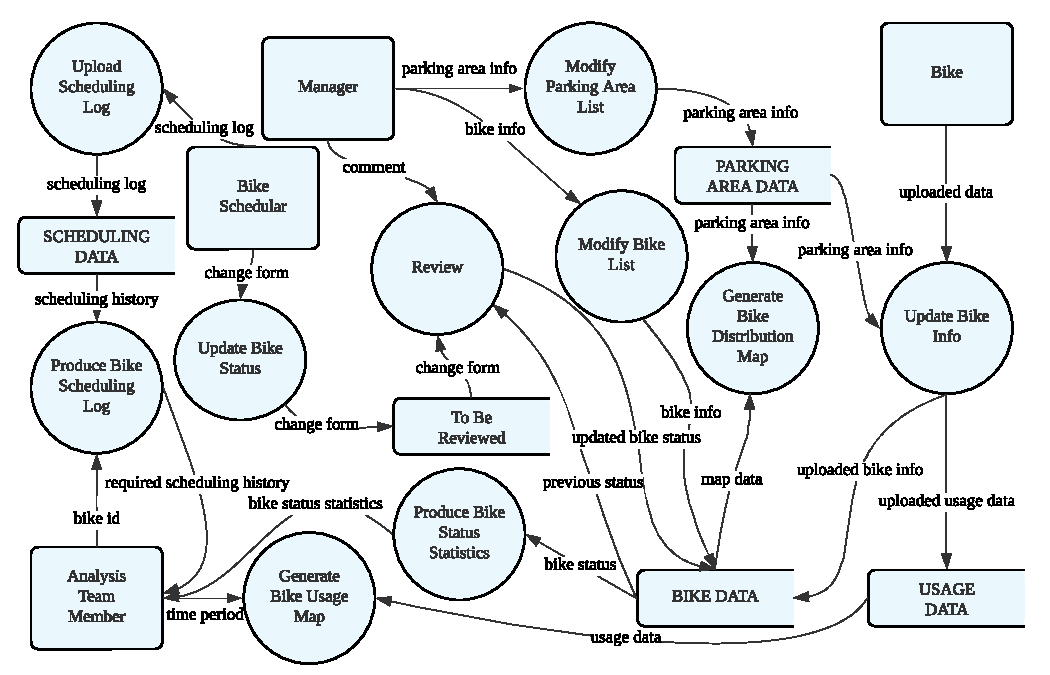
\includegraphics[width=\textwidth]{figures/DataFlow.pdf}
    \caption{数据流图}\label{DataFlow}
\end{figure}

\chapter{可行性分析}
\thispagestyle{empty}
\section{技术可行性}
从技术需求角度来看,本项目中所需的功能中比较具有挑战性的有:

\begin{enumerate}
    \item 利用地图进行可视化;
    \item 基于角色的鉴权;
    \item 在数据库中存储图片以及坐标数据。
\end{enumerate}

由于本项目使用基于\href{https://react.dev/}{React}的\href{https://nextjs.org/}{Next.js}框架,因此可以使用React生态来实现上述功能。\href{https://deck.gl/}{Deck.gl}提供了强大的地图可视化功能,\href{https://www.mapbox.com/}{mapbox}则提供了基础地图;
利用Next.js提供的cookies辅助函数可以方便地实现基于JWT的鉴权系统,从而实现基于角色的鉴权;PostGIS 是一个为 PostgreSQL 数据库提供地理信息系统(GIS)功能的扩展。
它将空间数据类型(如点、线、面等)和空间操作(如计算距离、面积、缓冲区分析等)引入 PostgreSQL。同时,Postgres支持TEXT类型的数据,因此我们可以将图片转为经Base64编码的字符串后
再存储至Postgres数据库中。

从技术需求方面来看,本项目涉及大量数据库的使用。为了尽可能地简化操控数据库的流程,同时提高数据的安全性,本项目使用\href{https://orm.drizzle.team/}{DrizzleORM}来访问数据库。
该ORM支持对于Point类型,适用于本项目。同时,本项目的另一挑战在于前端的设计。为此,本项目在使用Next.js的框架基础上,使用\href{https://tailwindcss.com/}{Tailwind CSS}和\href{https://nextui.org/}{NextUI}组件库,
大大提高网页开发的效率。

从开发周期上看,本项目有充足的时间以供增量式开发。

从技术风险角度来看,本项目使用的Next.js框架以及其他第三方方库均为最新版本,相对不稳定。但是Next.js以及本项目所采用的第三方库都拥有活跃的社区和积极
维护的开发人员,因此遇到的问题往往能够及时得到解决。

\section{应用可行性}

从部署角度上看,Next.js框架与\href{https://vercel.com/}{Vercel}部署平台深度绑定。项目开发完成后即可“一键”部署至云端。

从安全角度上看,该平台采用基于角色的鉴权方式,符合企业运营模式。同时,本项目中采用数据访问层(DAL),提高了数据访问的安全性,从而提高了该应用投入使用的可行性。
\chapter{概念设计}
\thispagestyle{empty}
\section{实体}
根据先前的需求分析,本系统所使用的数据库中,包含以下实体集:
\begin{itemize}
  \item \textit{bike}:拥有属性(\textit{\underline{bike\_ID},production\_date,coordinate,status,battery\_remaining\_capacity});
  \item \textit{usage}:拥有属性(\textit{\dotuline{time},coordinate,action});
  \item \textit{parking\_area}:拥有属性(\textit{\underline{parking\_area\_ID},name,coordinate,radius});
  \item \textit{scheduling}:拥有属性(\textit{\dotuline{time},coordinate,action});
  \item \textit{to\_be\_reviewed}:拥有属性(\textit{\dotuline{time},status,proof\_material});
\end{itemize}

\paragraph{\textit{bike}}

该实体集的拓展是在现实中公司所拥有的单车。

该实体集有以下属性:
\begin{itemize}
  \item \textit{\underline{bike\_ID}}:我们认为在同一家共享单车公司中,单车的序列号应当是唯一的,所以将其作为该实体集的主码;
  \item \textit{production\_date}:单车的生产日期;
  \item \textit{coordinate}:该属性用于追踪单车的当前坐标;
  \item \textit{status}:该属性用于记录单车状态,对应数据字典中的bike status项。
\end{itemize}

这里的\textit{production\_date,coordinate}实际上都是复合属性,例如\textit{coordinate}由经度和纬度组成,但是在该数据库的实际应用场景中,通常将它们
作为整体来使用,所以在概念设计中将它们视为整体。

这里的\textit{status}为多值属性,这是因为单车的实际状态可以由多个状态的合理组合而构成,例如一辆单车可以同时处于“闲置”和“低电量”状态。
\paragraph{\textit{usage}}

该实体集的拓展是在现实中共享单车用户对于共享单车的使用。

该实体集有以下属性:
\begin{itemize}
  \item \textit{\dotuline{time}}:事件发生时间;
  \item \textit{coordinate}:事件发生坐标;
  \item \textit{action}:该属性用于标记使用操作是开锁还是关锁;
\end{itemize}

我们认为共享单车的使用这一实体的存在依赖于单车实体。因此我将该实体集设计为弱实体集,它的识别集是\textit{bike},识别关系集是\textit{bike\_usage},识别器为该实体集的\textit{time}属性。

\paragraph{\textit{parking\_area}}

该实体集的拓展是在现实中公司所设立的停车地点。

该实体集有以下属性:
\begin{itemize}
  \item \textit{\underline{parking\_area\_ID}}:我们认为在同一家共享单车公司中,停车区域的ID号应当是唯一的,所以将其作为该实体集的主码;
  \item \textit{name}:停车区域名称;
  \item \textit{coordinate}:停车区域中心坐标;
  \item \textit{radius}:停车区域半径;
\end{itemize}

我们允许不同的停车区域有相同名称。
\paragraph{\textit{scheduling}}
该实体集的拓展是在现实中调度员所产生的调度行为。

该实体集有以下属性:
\begin{itemize}
  \item \textit{\dotuline{time}}:调度发生的时间;
  \item \textit{coordinate}:事件发生坐标;
  \item \textit{action}:该属性用于标记该事件是调度开始还是调度结束;
\end{itemize}
我们认为共享单车的调度这一实体的存在依赖于单车实体。因此我将该实体集设计为弱实体集,它的识别集是\textit{bike},识别关系集是\textit{bike\_scheduling},识别器为该实体集的\textit{time}属性。

\paragraph{\textit{to\_be\_reviewed}}

该实体集的拓展是在现实中调度员所提交的待审查更改。

该实体集有以下属性:
\begin{itemize}
  \item \textit{\dotuline{time}}:提交时间;
  \item \textit{status}:涉及单车状态;
  \item \textit{proof\_material}:用于证明单车状态更改合理性的图片;
\end{itemize}

我们认为待审核更改这一实体的存在依赖于单车实体。因此我将该实体集设计为弱实体集,它的识别集是\textit{bike},识别关系集是\textit{bike\_to\_be\_reviewed},识别器为该实体集的\textit{time}属性。

这里的\textit{status}为多值属性,这是因为单车的实际状态可以由多个状态的合理组合而构成,例如一辆单车可以同时处于“闲置”和“低电量”状态。
同时,\textit{proof\_material}也为多值属性,因为我们允许调度员上传多张照片来佐证状态改变的合理性。

\section{实体属性局部E-R图}

根据先前的需求分析,本系统所使用的数据库中,包含以下关系集:
\begin{itemize}
  \item \textit{bike\_usage}:将单车和单车使用记录关联在一起;
  \item \textit{contain}:将单车和单车停车区域关联在一起;
  \item \textit{bike\_scheduling}:将单车和单车调度记录关联在一起;
  \item \textit{bike\_to\_be\_reviewed}:将单车和待审查记录关联在一起;
\end{itemize}

\paragraph{\textit{bike\_usage}}
如图\ref{usage}所示,关系集\textit{bike\_usage}将实体集\textit{bike}与实体集\textit{usage}联系在一起。

该关系集表达的是“使用单车”这一事件中“单车”和“使用行为”之间的关系。这里的\textit{usage}是弱实体集,它的存在依附于实体集\textit{bike}。
因此,实体集\textit{usage}完全参与关系集\textit{bike\_usage}。

由于对于一次使用行为,有且仅有一辆单车与其相关联,而对于一辆单车,可能有多次使用行为与其相关联,所以图中有指向实体集\textit{bike}的箭头。
\begin{figure}[!htbp]
    \centering
    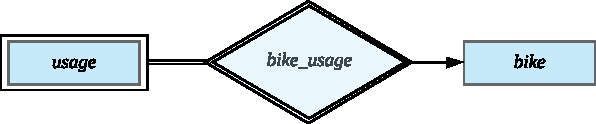
\includegraphics[scale=1]{figures/usage.pdf}
    \caption{\textit{bike\_usage}}\label{usage}
\end{figure}

\paragraph{\textit{contain}}
如图\ref{contain}所示,关系集\textit{contain}将实体集\textit{bike}与实体集\textit{parking\_area}联系在一起。

该关系集表达的是“单车停车区域”和“单车”之间的包含关系。

由于对于一个单车停车区域,可能包含多辆单车,而对于一辆单车,可能被多个停车区域所包含,所以图中并没有指向实体集的箭头。
\begin{figure}[!htbp]
    \centering
    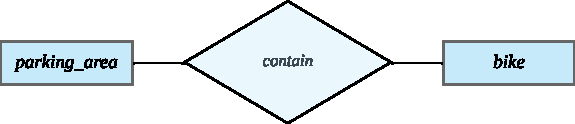
\includegraphics[scale=1]{figures/contain.pdf}
    \caption{\textit{contain}}\label{contain}
\end{figure}

\paragraph{\textit{bike\_scheduling}}

如图\ref{scheduling}所示,关系集\textit{bike\_scheduling}将实体集\textit{bike}与实体集\textit{scheduling}联系在一起。

该关系集表达的是“单车调度”这一事件中“单车”和“调度行为”之间的关系。这里的\textit{scheduling}是弱实体集,它的存在依附于实体集\textit{bike}。
因此,实体集\textit{scheduling}完全参与关系集\textit{bike\_scheduling}。

由于对于一次调度行为,可能涉及多辆单车,而对于一辆单车,也可能涉及多次调度行为,所以图中没有指向实体集的箭头。

\begin{figure}[!htbp]
    \centering
    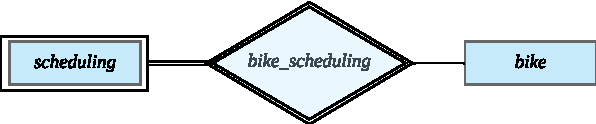
\includegraphics[scale=1]{figures/scheduling.pdf}
    \caption{\textit{bike\_scheduling}}\label{scheduling}
\end{figure}

\paragraph{\textit{to\_be\_reviewed}}
如图\ref{review}所示,关系集\textit{bike\_to\_be\_reviewed}将实体集\textit{bike}与实体集\textit{to\_be\_reviewed}联系在一起。

该关系集表达的是“提交待审查单车状态更新”这一事件中“单车”和“待审查单车状态更新”之间的关系。这里的\textit{to\_be\_reviewed}是弱实体集,它的存在依附于实体集\textit{bike}。
因此,实体集\textit{to\_be\_reviewed}完全参与关系集\textit{bike\_to\_be\_reviewed}。

由于对于一次待审查单车状态更新,有且仅有一辆单车与其相关联,而对于一辆单车,可能有多次待审查单车状态更新与其相关联,所以图中有指向实体集\textit{bike}的箭头。
\begin{figure}[!htbp]
    \centering
    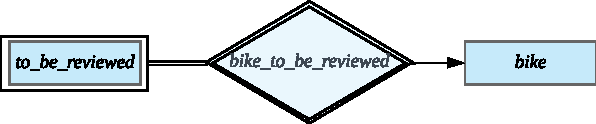
\includegraphics[scale=1]{figures/review.pdf}
    \caption{\textit{to\_be\_reviewed}}\label{review}
\end{figure}

\section{全局E-R图}
图\ref{ER}为全局E-R图。
\begin{figure}[!htbp]
    \centering
    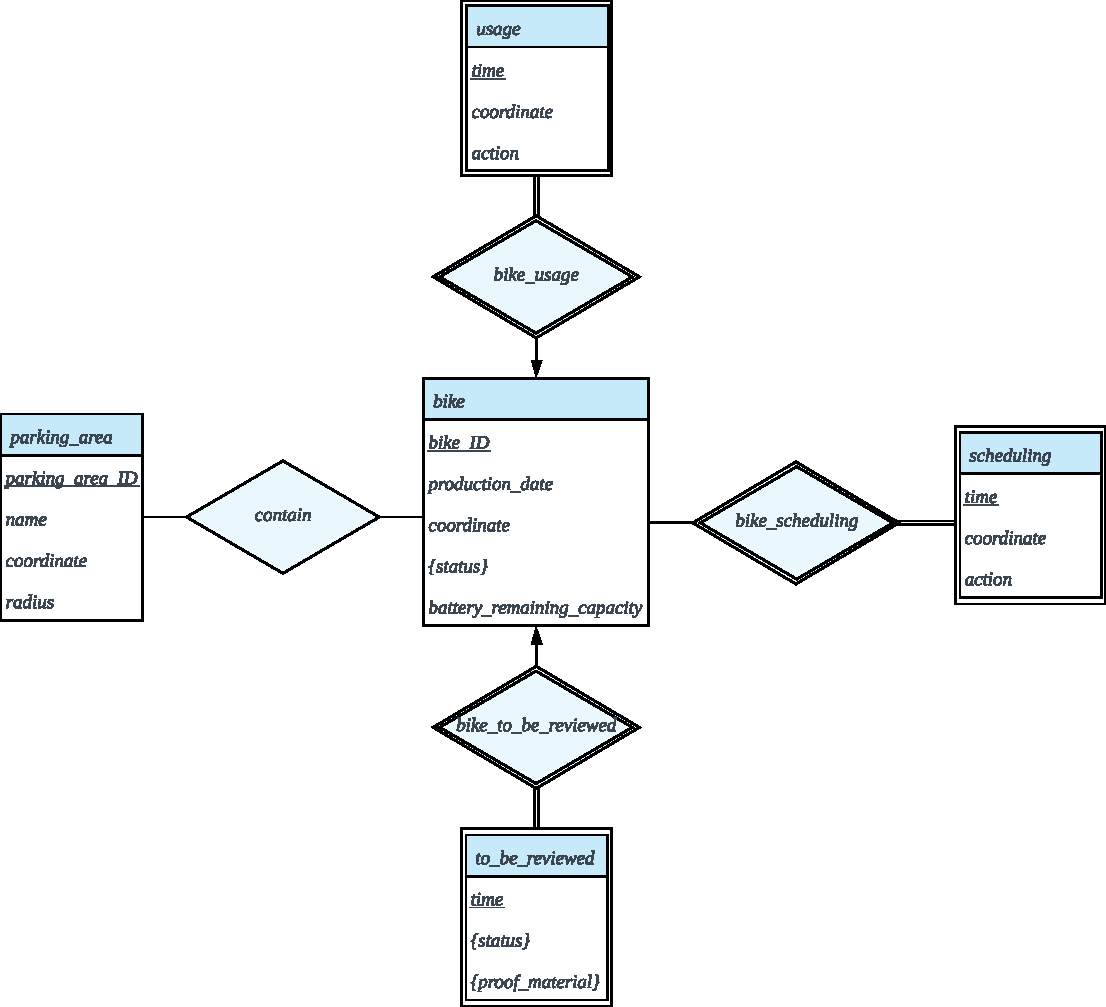
\includegraphics[width=\textwidth]{figures/ER.pdf}
    \caption{全局E-R图}\label{ER}
\end{figure}

\chapter{逻辑设计}
\thispagestyle{empty}
\section{E-R图向关系模型的转变}
\subsection{实体集模式}
\subsubsection{模式设计}
通过转换上述实体集,我们可以得到表\ref{tab:entityschema}中的实体集模式:
\begin{table}[!hpt]
    \caption{实体集模式}
    \label{tab:entityschema}
    \centering
    \begin{tabular}{l} \toprule
         \textit{bike}(\textit{\underline{bike\_ID},production\_date,coordinate,battery\_ramaining\_capacity})\\
         \textit{bike\_status}(\textit{\underline{bike\_ID},\underline{status}})\\
         \textit{usage}(\textit{\underline{bike\_ID},\underline{time},coordinate,action})\\
         \textit{parking\_area}(\textit{\underline{parking\_area\_ID},name,coordinate,radius})\\
         \textit{scheduling}(\textit{\underline{bike\_ID},\underline{time},coordinate,action})\\
         \textit{to\_be\_reviewed}(\textit{\underline{bike\_ID},\underline{time}})\\
         \textit{to\_be\_reviewed\_status}(\textit{\underline{bike\_ID},\underline{time},\underline{status}})\\
         \textit{to\_be\_reviewed\_proof\_material}(\textit{\underline{bike\_ID},\underline{time},\underline{no},proof\_material})\\\bottomrule
    \end{tabular}
  \end{table}

  在转换过程中,我们认为坐标、日期以及时间都是不可分割的单元。在实际应用场景中,也常常将它们作为整体来进行使用。

  对于弱实体集\textit{usage,scheduling}和\textit{to\_be\_reviewed},它们的模式的主码由自身的识别器\textit{time}和
  识别集的主码组成。

  对于实体集\textit{bike}中的属性\textit{status}和实体集\textit{to\_be\_reviewed}中的属性\textit{status}和\textit{proof\_material},它们是多值属性。
  为此,转换为模式时,额外创建模式\textit{bike\_status,to\_be\_reviewed\_status},\textit{to\_be\_}\\\textit{reviewed\_proof\_material}。
  模式\textit{bike\_status,to\_be\_reviewed\_status}的属性由原实集的主码和对应的多值属性组合而成,并且以它们作为主码。
  由于我们假设调度员可能会由于操作失误而上传多张相同的图片,同时,为了避免以图片数据作为主码的一部分,我们在模式\textit{to\_be\_reviewed\_proof\_material}中添加了\textit{no}域,用于表示证明材料的编号,并与
  \textit{bike\_ID,time}一同作为该模式的主码。
  
  对于其余强实体集,它们的模式的主码和属性与原来保持一致。

  \subsubsection{属性类型设计}
图\ref{tab:tobereviewedstatus}-\ref{tab:tobereviewedproofmaterial}为各实体集模式中属性的类型。
各类型定义与PostgreSQL文档\cite{data}一致。其中,\textbf{status}为自定义的枚举类型。

\begin{figure}[!htp]
    \begin{minipage}{0.33\textwidth}
      \centering
      \caption{\textit{to\_be\_reviewed\_status}属性类型}
      \label{tab:tobereviewedstatus}
      \begin{tabular}{ll}\toprule
        属性&类型\\\midrule
       \textit{bike\_ID}&\textbf{char}(20)\\
       \textit{time}&\textbf{timestamp}\\
       \textit{status}&\textbf{status}\\
       \bottomrule
      \end{tabular}



    \end{minipage}\hfill
    \begin{minipage}{0.33\textwidth}
      \centering
      \caption{\textit{bike\_status}属性类型}
      \label{tab:bikestatus}
      \begin{tabular}{ll}\toprule
        属性&类型\\\midrule
       \textit{bike\_ID}&\textbf{char}(20)\\
       \textit{status}&\textbf{status}\\
       \bottomrule
      \end{tabular}
    \end{minipage}\hfill
    \begin{minipage}{0.33\textwidth}
      \centering
      \caption{\textit{usage}属性类型}
      \label{tab:usage}
      \begin{tabular}{ll}\toprule
        属性&类型\\\midrule
       \textit{bike\_ID}&\textbf{char}(20)\\
       \textit{time}&\textbf{timestamp}\\
       \textit{coordinate}&\textbf{point}\\
       \textit{action}&\textbf{boolean}\\
       \bottomrule
      \end{tabular}
    \end{minipage}\hfill
  \end{figure}

\begin{figure}[!htp]
    \begin{minipage}{0.33\textwidth}
      \centering
      \caption{\textit{parking\_area}属性类型}
      \label{tab:parkingarea}
      \begin{tabular}{ll}\toprule
        属性&类型\\\midrule
       \textit{parking\_area\_ID}&\textbf{serial}\\
       \textit{name}&\textbf{char}(20)\\
       \textit{coordinate}&\textbf{point}\\
       \textit{radius}&\textbf{real}\\
       \bottomrule
      \end{tabular}
    \end{minipage}\hfill
    \begin{minipage}{0.33\textwidth}
      \centering
      \caption{\textit{scheduling}属性类型}
      \label{tab:scheduling}
      \begin{tabular}{ll}\toprule
        属性&类型\\\midrule
       \textit{bike\_ID}&\textbf{char}(20)\\
       \textit{time}&\textbf{timestamp}\\
       \textit{coordinate}&\textbf{point}\\
       \textit{action}&\textbf{boolean}\\
       \bottomrule
      \end{tabular}
    \end{minipage}\hfill
    \begin{minipage}{0.33\textwidth}
      \centering
      \caption{\textit{to\_be\_reviewed}属性类型}
      \label{tab:tobereviewed}
      \begin{tabular}{ll}\toprule
        属性&类型\\\midrule
       \textit{bike\_ID}&\textbf{char}(20)\\
       \textit{time}&\textbf{timestamp}\\
       \bottomrule
      \end{tabular}
    \end{minipage}\hfill
  \end{figure}

\begin{figure}[!htp]
    \begin{minipage}{0.5\textwidth}
      \centering

      \caption{\textit{bike}属性类型}
      \label{tab:bike}
      \begin{tabular}{ll}\toprule
        属性&类型\\\midrule
       \textit{bike\_ID}&\textbf{char}(20)\\
       \textit{production\_date}&\textbf{date}\\
       \textit{coordinate}&\textbf{point}\\
       \textit{battery\_remaining\_capacity}&\textbf{real}\\
       \bottomrule
      \end{tabular}

    \end{minipage}\hfill
    \begin{minipage}{0.5\textwidth}
      \centering
      \caption{\textit{to\_be\_reviewed\_proof\_material}属性类型}
      \label{tab:tobereviewedproofmaterial}
      \begin{tabular}{ll}\toprule
        属性&类型\\\midrule
       \textit{bike\_ID}&\textbf{char}(20)\\
       \textit{time}&\textbf{timestamp}\\
       \textit{no}&\textbf{smallint}\\
       \textit{proof\_material}&\textbf{text}\\
       \bottomrule
      \end{tabular}
    \end{minipage}\hfill
  \end{figure}
\subsection{关系集模式}
\subsubsection{模式设计}
  通过转换上述关系集,我们可以得到表\ref{tab:relationschema}中的关系集模式:

  \begin{table}[!hpt]
      \caption{关系集模式}
      \label{tab:relationschema}
      \centering
      \begin{tabular}{l} \toprule
           \textit{contain}(\textit{\underline{bike\_ID},\underline{parking\_area\_ID}})\\
           \bottomrule
      \end{tabular}
    \end{table}

    在转换的过程中,联系弱实体集和其对应识别集的关系集\textit{bike\_usage,bike\_scheduling}和\textit{bike\_to\_be\_reviewed}被略去,因为这是冗余的\cite{dbconcept2}。

    关系集\textit{contain}为“多对多”的二元关系集,其模式的主码由它关联起来的实体集模式的主码组合而成。

\subsubsection{属性类型设计}
  关系集模式中属性的类型与实体集中的相应属性类型保持一致。图\ref{tab:contain}为\textit{contain}模式中属性的类型。
  \begin{figure}[!htp]
      \centering
      \caption{\textit{contain}属性类型}
      \label{tab:contain}
      \begin{tabular}{ll}\toprule
        属性&类型\\\midrule
       \textit{bike\_ID}&\textbf{char}(20)\\
       \textit{parking\_area\_ID}&\textbf{serial}\\
       \bottomrule
      \end{tabular}
\end{figure}
\subsection{约束设计}
图\ref{contraint:bike}-\ref{contraint:tobereviewedproofmaterial}为各模式中的属性所需遵循的约束。

约束设计主要分为两部分:外码约束和其他约束。

\paragraph{外码约束}
外码约束主要有三个来源:

\begin{enumerate}
    \item 关系集转化为关系集模式时所产生的;
    \item 转化复杂类型时所产生的;
    \item 转化弱实体集时所产生的。
\end{enumerate}

在本数据库中,由于多值属性而额外生成的模式\textit{bike\_status,to\_be\_reviewed\_status,to\_be\_}\\\textit{reviewed\_proof\_material}与原模式之间存在外码约束。
它们的主码需引用原模式的主码。

弱实体集\textit{usage,scheduling,to\_be\_reviewed}转换为模式时,需遵循外码约束,引用其识别集的主码。

其余外码约束来自于由关系集\textit{contain}转化而来的关系集模式,需要引用模式\textit{parking\_area}与\textit{bike}的主码。

\paragraph{其他约束}
本数据库中的其他约束包括主码约束(非空且唯一)、非空约束、唯一约束和CHECK约束。

由于本数据库中除了\textit{proof\_material,radius}外的其他所有域理论上都可以由相应的设备自动生成,如电池剩余电量,又或者是必不可少的一部分,例如停车区域半径,所以所有属性都遵循非空约束。

对于坐标、时间戳、证明材料等数据,我们不作唯一约束要求。

在本数据库中,CHECK约束主要用于确保停车区域半径大于一定值,我们假设停车区域半径至少大于10米。

特别地,\textit{text}表中的记录与“违规停车”在语义上有着直接关联。我们规定一辆单车当且仅当不出现在\textit{text}表中时拥有“违规停车”状态。
为了维护该约束,我们采用触发器。

\begin{figure}[!htp]
      \centering
      \caption{\textit{bike}属性约束}
      \label{contraint:bike}
      \begin{tabular}{ll}\toprule
        属性&约束\\\midrule
       \textit{bike\_ID}&\textbf{PRIMIARY KEY}\\
       \textit{production\_date}&\textbf{NOT NULL}\\
       \textit{coordinate}&\textbf{NOT NULL}\\
       \textit{battery\_remaining\_capacity}&\makecell[l]{\textbf{CHECK} \textit{battery\_remaining\_capacity between 0 AND 1}\\\textbf{NOT NULL}}\\
       \bottomrule
      \end{tabular}
\end{figure}

\begin{figure}[!htp]
    \begin{minipage}{0.5\textwidth}
      \centering
      \caption{\textit{to\_be\_reviewed\_status}属性约束}
      \label{contraint:tobereviewedstatus}
      \begin{tabular}{ll}\toprule
        属性&约束\\\midrule
       \textit{bike\_ID}&\textbf{REFERENCES} \textit{bike}\\
       \textit{time}&\\
       \textit{status}&\\
       \textit{(bike\_ID,time,status)}&\textbf{PRIMIARY KEY}\\
       \bottomrule
      \end{tabular}
    \end{minipage}\hfill
    \begin{minipage}{0.5\textwidth}
      \centering
      \caption{\textit{bike\_status}属性约束}
      \label{contraint:bikestatus}
      \begin{tabular}{ll}\toprule
        属性&约束\\\midrule
       \textit{bike\_ID}&\textbf{REFERENCES} \textit{bike}\\
       \textit{status}&\\
       \textit{(bike\_ID,status)}&\textbf{PRIMIARY KEY}\\
       \bottomrule
      \end{tabular}
    \end{minipage}\hfill
 \end{figure}

\begin{figure}[!htp]
    \begin{minipage}{0.5\textwidth}
      \centering
      \caption{\textit{usage}属性约束}
      \label{contraint:usage}
      \begin{tabular}{ll}\toprule
        属性&约束\\\midrule
       \textit{bike\_ID}&\\
       \textit{time}&\\
       \textit{coordinate}&\textbf{NOT NULL}\\
       \textit{action}&\textbf{NOT NULL}\\
       \textit{(bike\_ID,time)}&\textbf{PRIMIARY KEY}\\
       \textit{(bike\_ID,time)}&\textbf{REFERENCES} \textit{bike\_status}\\
       \bottomrule
      \end{tabular}
    \end{minipage}\hfill
    \begin{minipage}{0.5\textwidth}
      \centering
      \caption{\textit{parking\_area}属性约束}
      \label{contraint:parkingarea}
      \begin{tabular}{ll}\toprule
        属性&约束\\\midrule
       \textit{parking\_area\_ID}&\textbf{PRIMIARY KEY}\\
       \textit{name}&\textbf{NOT NULL}\\
       \textit{coordinate}&\textbf{NOT NULL}\\
       \textit{radius}&\makecell[l]{\textbf{CHECK} \textit{radius>=10}\\\textbf{NOT NULL}}\\
       \bottomrule
      \end{tabular}
    \end{minipage}\hfill
 \end{figure}


\begin{figure}[!htp]
      \centering
      \caption{\textit{contain}属性约束}
      \label{contraint:contain}
      \begin{tabular}{ll}\toprule
        属性&约束\\\midrule
       \textit{bike\_ID}&\textbf{REFERENCES} \textit{bike}\\
       \textit{parking\_area\_ID}&\textbf{REFERENCES} \textit{parking\_area}\\
       \textit{(bike\_ID,parking\_area\_ID)}&\textbf{PRIMIARY KEY}\\
       \bottomrule
      \end{tabular}
\end{figure}

\begin{figure}[!htp]
    \begin{minipage}{0.5\textwidth}
      \centering
      \caption{\textit{scheduling}属性约束}
      \label{contraint:scheduling}
      \begin{tabular}{ll}\toprule
        属性&约束\\\midrule
       \textit{bike\_ID}&\textbf{REFERENCES} \textit{bike}\\
       \textit{time}&\\
       \textit{coordinate}&\textbf{NOT NULL}\\
       \textit{action}&\textbf{NOT NULL}\\
       \textit{(bike\_ID,time)}&\textbf{PRIMIARY KEY}\\
       \bottomrule
      \end{tabular}
    \end{minipage}\hfill
    \begin{minipage}{0.5\textwidth}
      \centering
      \caption{\textit{to\_be\_reviewed}属性约束}
      \label{contraint:tobereviewed}
      \begin{tabular}{ll}\toprule
        属性&约束\\\midrule
       \textit{bike\_ID}&\textbf{REFERENCES} \textit{bike}\\
       \textit{time}&\\
       \textit{(bike\_ID,time)}&\textbf{PRIMIARY KEY}\\
       \bottomrule
      \end{tabular}
    \end{minipage}\hfill
\end{figure}


\begin{figure}[!htp]

      \centering
      \caption{\textit{to\_be\_reviewed\_proof\_material}属性约束}
      \label{contraint:tobereviewedproofmaterial}
      \begin{tabular}{ll}\toprule
        属性&约束\\\midrule
       \textit{bike\_ID}&\\
       \textit{time}&\\
       \textit{no}&\textbf{CHECK} no>=0\\
       \textit{proof\_material}&\textbf{NOT NULL}\\
       \textit{(bike\_ID,time,no)}&\textbf{PRIMIARY KEY}\\
       \textit{(bike\_ID,status)}&\textbf{REFERENCES} \textit{bike\_status}\\
       \bottomrule
      \end{tabular}

\end{figure}

\subsection{模式图}

图\ref{schema}为本系统所用数据库的模式图。

\begin{figure}[!htbp]
    \centering
    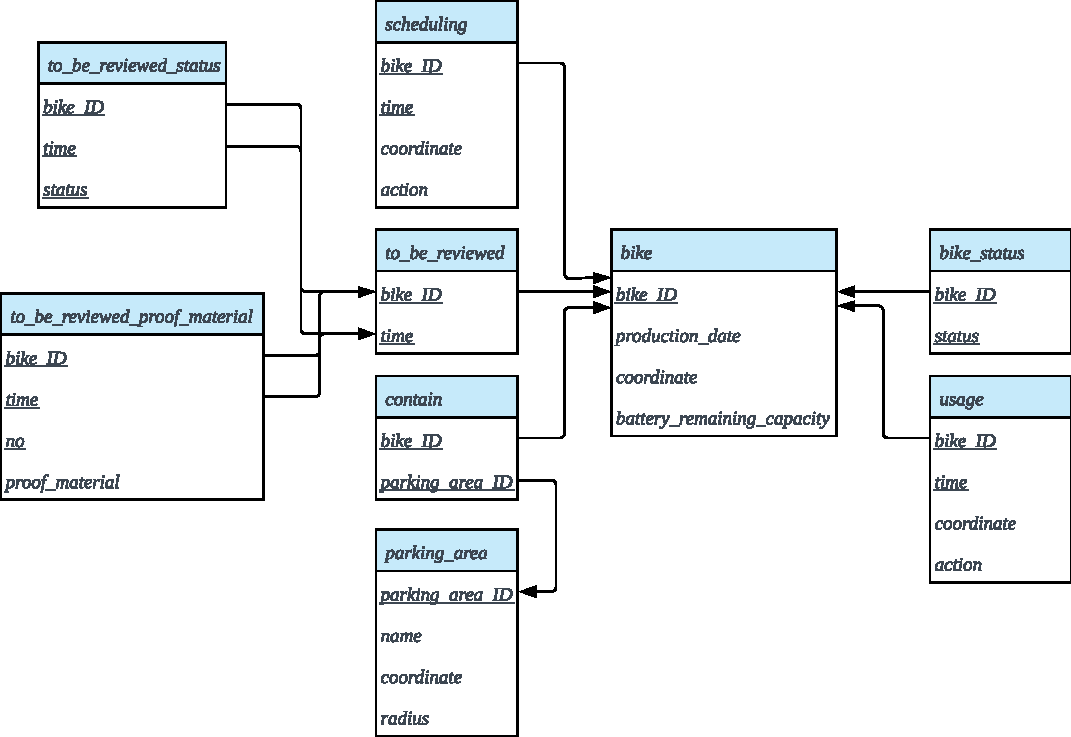
\includegraphics[width=\textwidth]{figures/schema.pdf}
    \caption{模式图}\label{schema}
\end{figure}

\section{数据模型的优化及规范化设计}

\subsection{第一范式}
在从E-R图转换至模式的过程中,我已经将复杂属性拆分开来,所以所有模式满足第一范式。
\subsection{第二范式}
\begin{table}[!hpt]
  \caption{各模式中的函数依赖的正则覆盖}
  \label{tab:functiondependency}
  \centering
  \begin{tabular}{l} \toprule
      $FC_{scheduling}=\{\{bike\_ID,time\}\rightarrow \{coordinate,action\}\}$\\
      $FC_{to\_be\_reviewed}=\varnothing$\\
      $FC_{contain}=\varnothing$\\
      $FC_{parking\_area}=\{parking\_area\_ID\rightarrow \{name,coordinate,radius\}\}$\\
      $FC_{bike}=\{bike\_ID\rightarrow \{production\_date,coordinate,battery\_remaining\_capacity \}\}$\\
      $FC_{to\_be\_reviewed\_proof\_material}=\{\{bike\_ID,time,no\}\rightarrow proof\_material\}$\\
      $FC_{to\_be\_reviewed\_status}=\varnothing$\\
      $FC_{bike\_status}=\varnothing$\\
      $FC_{usage}=\{\{bike\_ID,time\}\rightarrow\{coordinate,action\}\}$\\
       \bottomrule
  \end{tabular}
\end{table}

经过验证,各个模式中不存在部分函数依赖,即所有模式满足第二范式。
\subsection{第三范式}
经过验证,各个模式中不存在传递依赖的关系,即所有模式满足第三范式。
\subsection{BC范式}
经过验证,所有模式满足BC范式。

\chapter{项目管理}
\thispagestyle{empty}
\section{框架选择}
本项目采用Next.js作为全栈框架。它是一个开源的 JavaScript 框架,基于 React 构建,旨在简化和优化现代 Web 应用的开发。它提供了很多开箱即用的功能,能够帮助开发者构建快速、可扩展的 Web 应用,尤其适用于静态网站生成(SSG)、服务器端渲染(SSR)和客户端渲染(CSR)。

Next.js具有以下特点:
\begin{enumerate}
    \item \textbf{服务器端渲染(SSR)}:
    Next.js 支持服务器端渲染,这意味着页面的 HTML 可以在服务器上预先渲染,然后传送给客户端。这有助于提高 SEO(搜索引擎优化)性能,因为搜索引擎可以直接读取渲染好的 HTML。
    
    \item \textbf{静态站点生成(SSG)}:
    Next.js 支持通过静态站点生成(SSG)功能,在构建时生成静态 HTML 页面。这对于内容更新不频繁的应用非常有效,能显著提高性能。
    
    \item \textbf{API 路由}:
    Next.js 可以用来构建 API 服务,允许开发者在同一个项目中同时处理前端和后端逻辑。开发者可以在 \texttt{pages/api} 目录下创建 API 路由,从而处理服务器端的请求。
    
    \item \textbf{增量静态生成(ISR)}:
    Next.js 提供了增量静态生成功能,允许开发者在生产环境中动态地更新静态页面。开发者可以设置页面的重新生成周期,这对于需要定期更新内容的应用非常有用。
    
    \item \textbf{自动代码拆分}:
    Next.js 会自动拆分 JavaScript 代码,按需加载页面,确保每个页面只加载它需要的 JavaScript,提升页面加载速度。
    
    \item \textbf{文件系统路由}:
    在 Next.js 中,路由是基于文件系统的。只要在 \texttt{pages} 目录下创建相应的文件或目录,就会自动生成对应的路由。
    
    \item \textbf{静态文件支持}:
    Next.js 允许开发者将静态文件(如图片、字体、JSON 等)放置在 \texttt{public} 目录中,并自动生成可访问的 URL。
    
    \item \textbf{类型支持}:
    Next.js 完全支持 TypeScript,可以直接在项目中使用 TypeScript,无需额外配置。
    
    \item \textbf{React 特性}:
    由于 Next.js 基于 React,开发者可以利用 React 的所有特性,如组件化开发、Hooks、Context 等。
\end{enumerate}
\section{开发平台}
本项目使用的开发平台如下:
\begin{itemize}
    \item \textbf{开发语言}:TypeScript;
    \item \textbf{开发框架}:采用Next.js作为全栈框架;
    \item \textbf{集成开发环境}:VSCode,WebStorm;
    \item \textbf{版本控制工具}:Git;
    \item \textbf{前期设计工具}:Adobe XD;
    \item \textbf{代码托管平台}:GitHub;
    \item \textbf{依赖管理工具}:pnpm;
    \item \textbf{数据库管理工具}:DataGrip,pgAdmin4;
    \item \textbf{数据库}:PostgreSQL+PostGIS;
    \item \textbf{ORM框架}:DrizzleORM;
    \item \textbf{CSS框架}:Tailwind CSS;
    \item \textbf{组件库}:NextUI;
    \item \textbf{地理空间数据可视化平台}:Deck.gl,Mapbox;
\end{itemize}
\chapter{项目实现}
\thispagestyle{empty}
\section{项目框架搭建}
%概述整个系统的架构
整个系统使用Next.js进行全栈开发。

对于前端,我使用Next.js,React和NextUI来构建页面和组件。使用Tailwind CSS进行样式设计,编写的组件集中在 \verb|src\ui|文件夹中。
同时,我使用Next.js了最新推出的文件系统路由,在\verb|src/app/|目录下构建页面和布局,每个\verb|page.tsx|文件自动映射
到网页,每个\verb|layout.tsx|文件自动映射到网页布局。
其中, \texttt{dashboard}文件夹对应的是单车与停车区域分布页面,用于实现用例\texttt{Generate Bike Distribution Map}和\texttt{Generate Parking Area Distribution Map};
\texttt{scheduleMap}文件夹对应的是查询调度记录页面,用于实现用例\texttt{Produce Bike Scheduling Log}; \texttt{usageMap}文件夹对应的是使用记录图页面,用于实现用例\texttt{Generate Bike Usage Map};
\texttt{modifyPanel}文件夹对应的是修改数据页面,用于实现用例\texttt{Modify Bike List},\texttt{Modify Parking Area List},\texttt{Update Bike Status Globally}; \texttt{reviewPanel}文件夹对应的是审查页面,用于实现用例\texttt{Update Single Bike Status}; \texttt{login}文件夹对应的是登录页面; \texttt{app}文件夹对应的是欢迎页面。
特别地, \texttt{api}文件夹对应的是开放给单车和调度员上传数据的API接口,其中 \texttt{bike}文件夹对应的是用于接收单车所上传信息的接口,用于实现用例\texttt{Update Bike Information}; \texttt{changeForm}文件夹对应的是
用于接收调度员所上传的修改状态数据的接口,用于实现\texttt{Update Single Bike Status}; \texttt{schedulingLog}文件夹对应的是用于接收调度员上传的调度记录的接口,用于实现用例\texttt{Upload Scheduling Log}。

对于后端,绝大部分的功能,如用户认证、表单提交和数据处理,我都通过Next.js提供的Server Actions功能来实现。
所编写的Server Actions集中在\verb|src\lib\actions.ts|中。对于调度员和单车上传数据的需求,我仍然通过API路由来
接受他们所上传的信息,但是后续的处理仍然是通过Server Actions来实现。在数据管理部分,我通过Drizzle ORM
与Postgres数据库进行交互,并且通过数据访问层(DAL)来保障数据安全,相关的代码集中在\verb|src\lib\dal.ts|中。

在本项目中,我通过数据库管理工具DataGrip来直接运行位于\texttt{init}文件夹下的\texttt{init.sql}文件以初始化数据库。

\section{系统逻辑设计}
%系统的功能实现逻辑
\subsection{业务逻辑}
本项目的业务逻辑按照图\ref{GenerateBikeDistributionMap}-\ref{ModifyParkingAreaList}中的用例说明来实现,这里不再赘述。
\subsection{基于角色的鉴权}
本项目中利用JWT来实现基于角色的鉴权。运行逻辑如下:

\begin{enumerate}
        \item 用户登录时,要求输入邮箱和密码
        \item 将邮箱和密码与数据库中存储的数据进行对比,若无匹配项,则重定向至登录页,并进行提示;若成功匹配,则将用户的角色保存至会话中;
        \item 系统将生成的 JWT 存储为 cookie,作为会话凭据;
        \item 系统在中间件\verb|src\middleware.ts|中设计了更新会话的过期时间的机制,以确保用户的会话在活跃期间不会过期;
        \item 在渲染修改数据页面和审查页面之前,会检查会话中保存的角色是否为 \verb|MANAGER|;在数据访问层中与数据库交互之前,会检查会话凭据是否有效;
        \item 若用户越权访问,则会重定向至提示页;若用户的会话凭据过期,系统会要求用户重新登录;
        \item 当用户登出时,系统会清除存储在cookie中的会话凭据,并将用户重定向至登录页面。
\end{enumerate}

% \begin{figure}[!htbp]
%     \centering
%     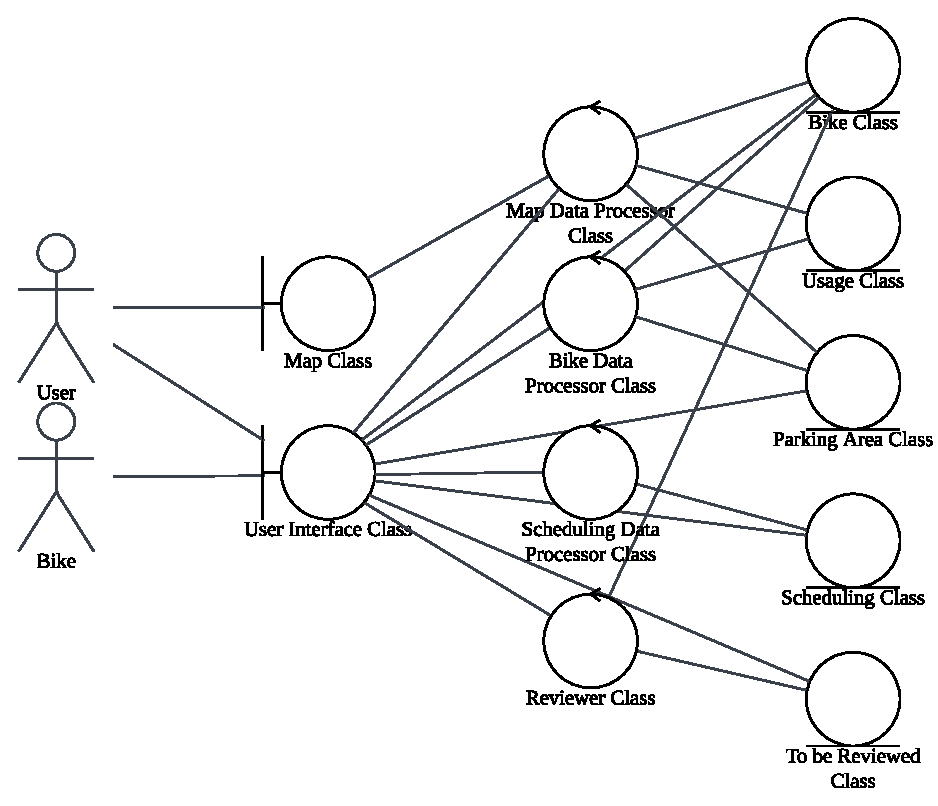
\includegraphics[width=\textwidth]{figures/class.pdf}
%     \caption{类图}\label{class}
% \end{figure}

\section{具体功能编写}
%简单介绍系统编写过程
在本项目的开发过程中,我们先使用Adobe XD来确定整个系统前端的设计和交互逻辑,然后使用Tailwind CSS和NextUI来
快速搭建出前端页面。

对于后端开发,由于本项目所采用的是Typescript语言,所以我首先根据数据字典来编写包含本项目所需类型定义的文件\verb|src\lib\definitions.ts|。
在此基础之上,再根据数据流图编写数据访问层对应文件\verb|src\lib\dal.ts|。最后,根据用例中描述的逻辑来实现业务逻辑,在此过程中完成Server Actions对应文件
\verb|src\lib\actions.ts|的编写。当然,在实际的开发过程中,上述三个部分相互之间是穿插着进行的,但是大体流程仍是分为上述三个阶段。

特别地,我在数据库中创建以下用户自定义函数:

\begin{enumerate}
    \item \texttt{create\_manager}:用户创建管理员账号;
    \item \texttt{create\_analyst}:用于创建分析团队账号;
    \item \texttt{check\_password}:用于检查账号和密码是否正确;
    \item \texttt{mark\_low\_battery}:用于全局更新“低电量”状态;
    \item \texttt{mark\_idle\_bikes}:用于全局更新“闲置”状态;
    \item \texttt{update\_luflt\_status}:用于全局更新“长期未关锁”状态;
    \item \texttt{update\_outdated\_status}:用于全局更新“型号老旧”状态;
    \item \texttt{update\_on\_parking\_area\_change}:给定停车区域数据,更新与该数据相关的\verb|contain|表中的数据,以及“违规停车”状态;
    \item \texttt{update\_on\_bike\_change}:给定单车数据,更新与该数据相关的\verb|contain|表中的数据,以及“违规停车”状态;
\end{enumerate}

同时,我在数据库中创建了以下触发器:

\begin{enumerate}
    \item \texttt{trigger\_parking\_area}:当管理创建、删除或更新停车区域数据时,自动对涉及数据调用 \texttt{update\_on\_parking\_area\_change}来维护一致性;
    \item \texttt{trigger\_bike}:当共享单车上传数据,或者管理员更新、创建或删除单车数据时,自动对涉及数据调用\texttt{update\_on\_bike\_change}来维护一致性;
\end{enumerate}

在项目开发末尾,我对本系统对于数据库的交互进行了统计分析。并对频繁用于连接和条件查询的域建立了索引。


\begin{table}
\centering
\caption{索引}
\label{index}
\begin{tabular}{ll}\toprule
  索引名&索引对象\\\midrule
  \texttt{idx\_scheduling}&\textit{\textbf{scheduling}(bike\_id)}\\
  \texttt{idx\_bike\_status}&\textit{\textbf{bike\_status}(bike\_id)}\\
  \texttt{idx\_parking\_area}&\textit{\textbf{parking\_area}(parking\_area\_id)}\\
  \texttt{idx\_bike}&\textit{\textbf{bike}(bike\_id)}\\
  \texttt{idx\_to\_be\_reviewed\_status}&\textit{\textbf{to\_be\_reviewed\_status}(bike\_id,time)}\\
  \texttt{idx\_to\_be\_reviewed\_proof\_material}&\textit{\textbf{to\_be\_reviewed\_proof\_material}(bike\_id,time)}\\
  \texttt{idx\_to\_be\_reviewed}&\textit{\textbf{to\_be\_reviewed}(bike\_id,time)}\\
  \texttt{idx\_usage}&\textit{\textbf{usage}(bike\_id)}\\
  \texttt{idx\_contain}&\textit{\textbf{contain}(bike\_id)}\\
  \texttt{idx\_contain\_}&\textit{\textbf{contain}(parking\_area\_id)}\\
 \bottomrule
\end{tabular}
\end{table}

\section{功能测试}
% %对编写系统进行实际测试
我对系统进行两方面的测试:

\begin{enumerate}
    \item 以摩拜共享单车2017年8月的数据集为基础,构造数据,并对数据库进行填充,主要用于测试用例\texttt{Generate Bike Distribution Map},\texttt{Generate Parking Area Distribution Map},\texttt{Produce Bike Status Statistics},\texttt{Update Bike Status Globally};
    \item 使用空数据库,主要用于测试涉及插入操作的用例,如\texttt{Upload Scheduling Log},\texttt{Update Single Bike Status},\texttt{Produce Bike Scheduling Log},\texttt{Update Bike Information},\texttt{Modify Bike List},\texttt{Modify Parking Area List}。
\end{enumerate}

上述两个测试覆盖了本项目的所有用例。

系统成功通过测试,并无功能性缺陷,但是在响应时间方面还有提升空间。测试时系统页面如图\ref{dashboard}-\ref{reviewPage}所示。

\begin{figure}[!htbp]
    \centering
    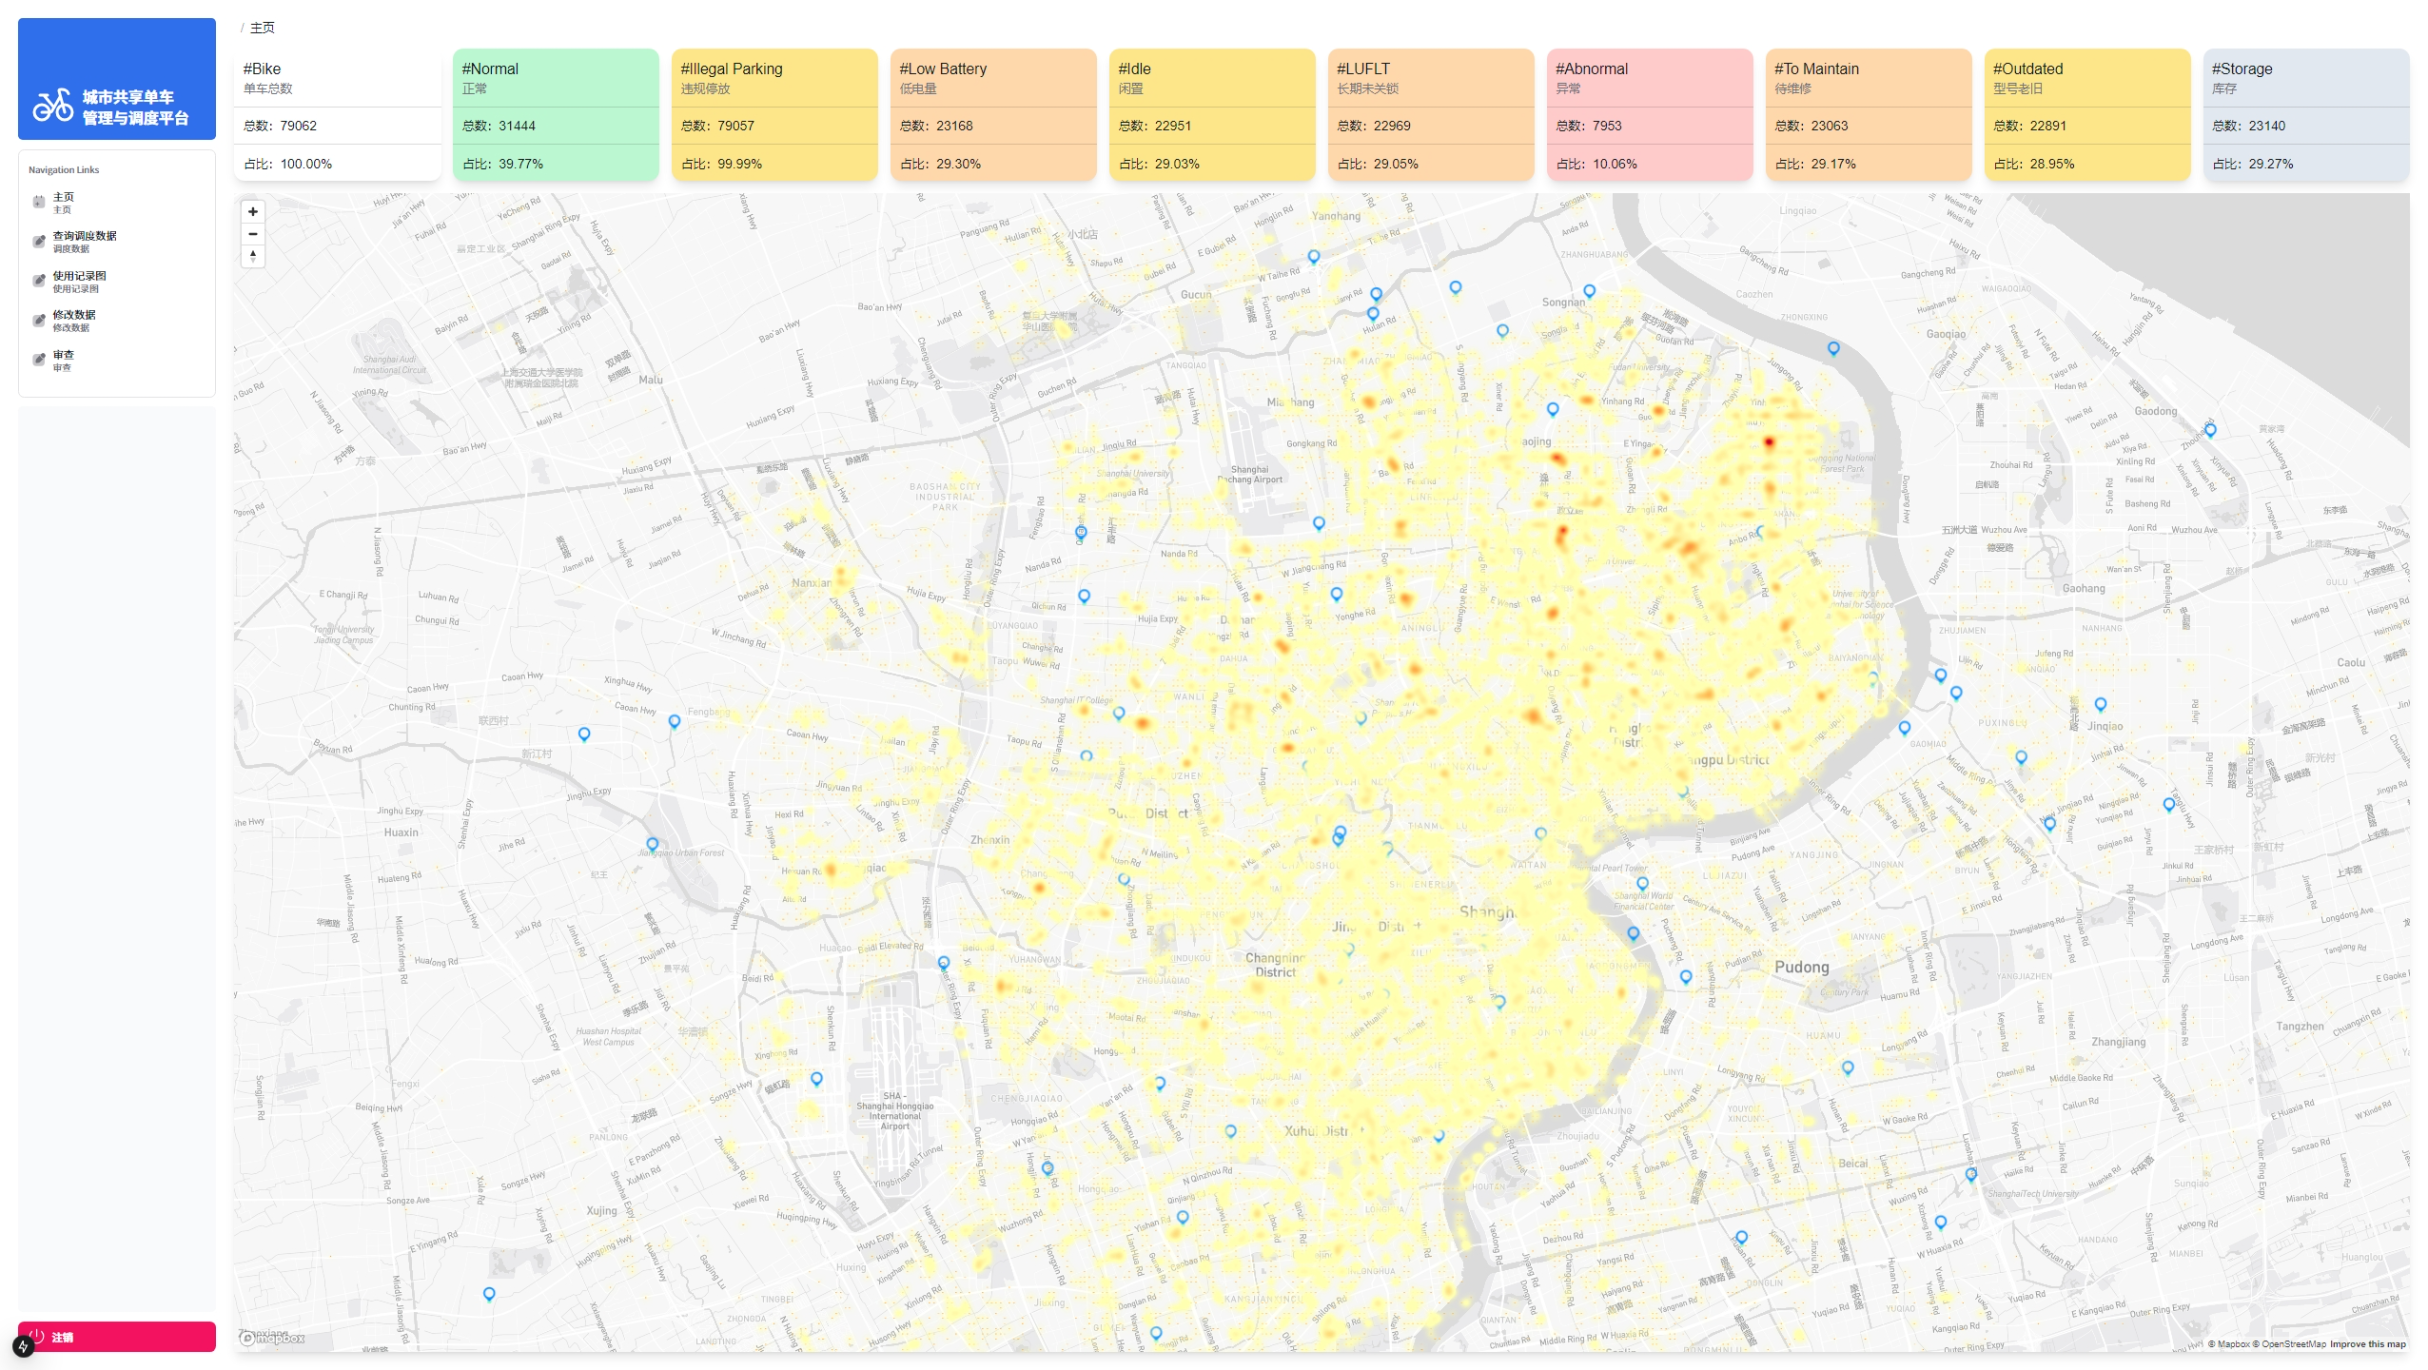
\includegraphics[width=\textwidth]{figures/dashboard.png}
    \caption{单车与停车区域分布图}\label{dashboard}
\end{figure}

\begin{figure}[!htbp]
    \centering
    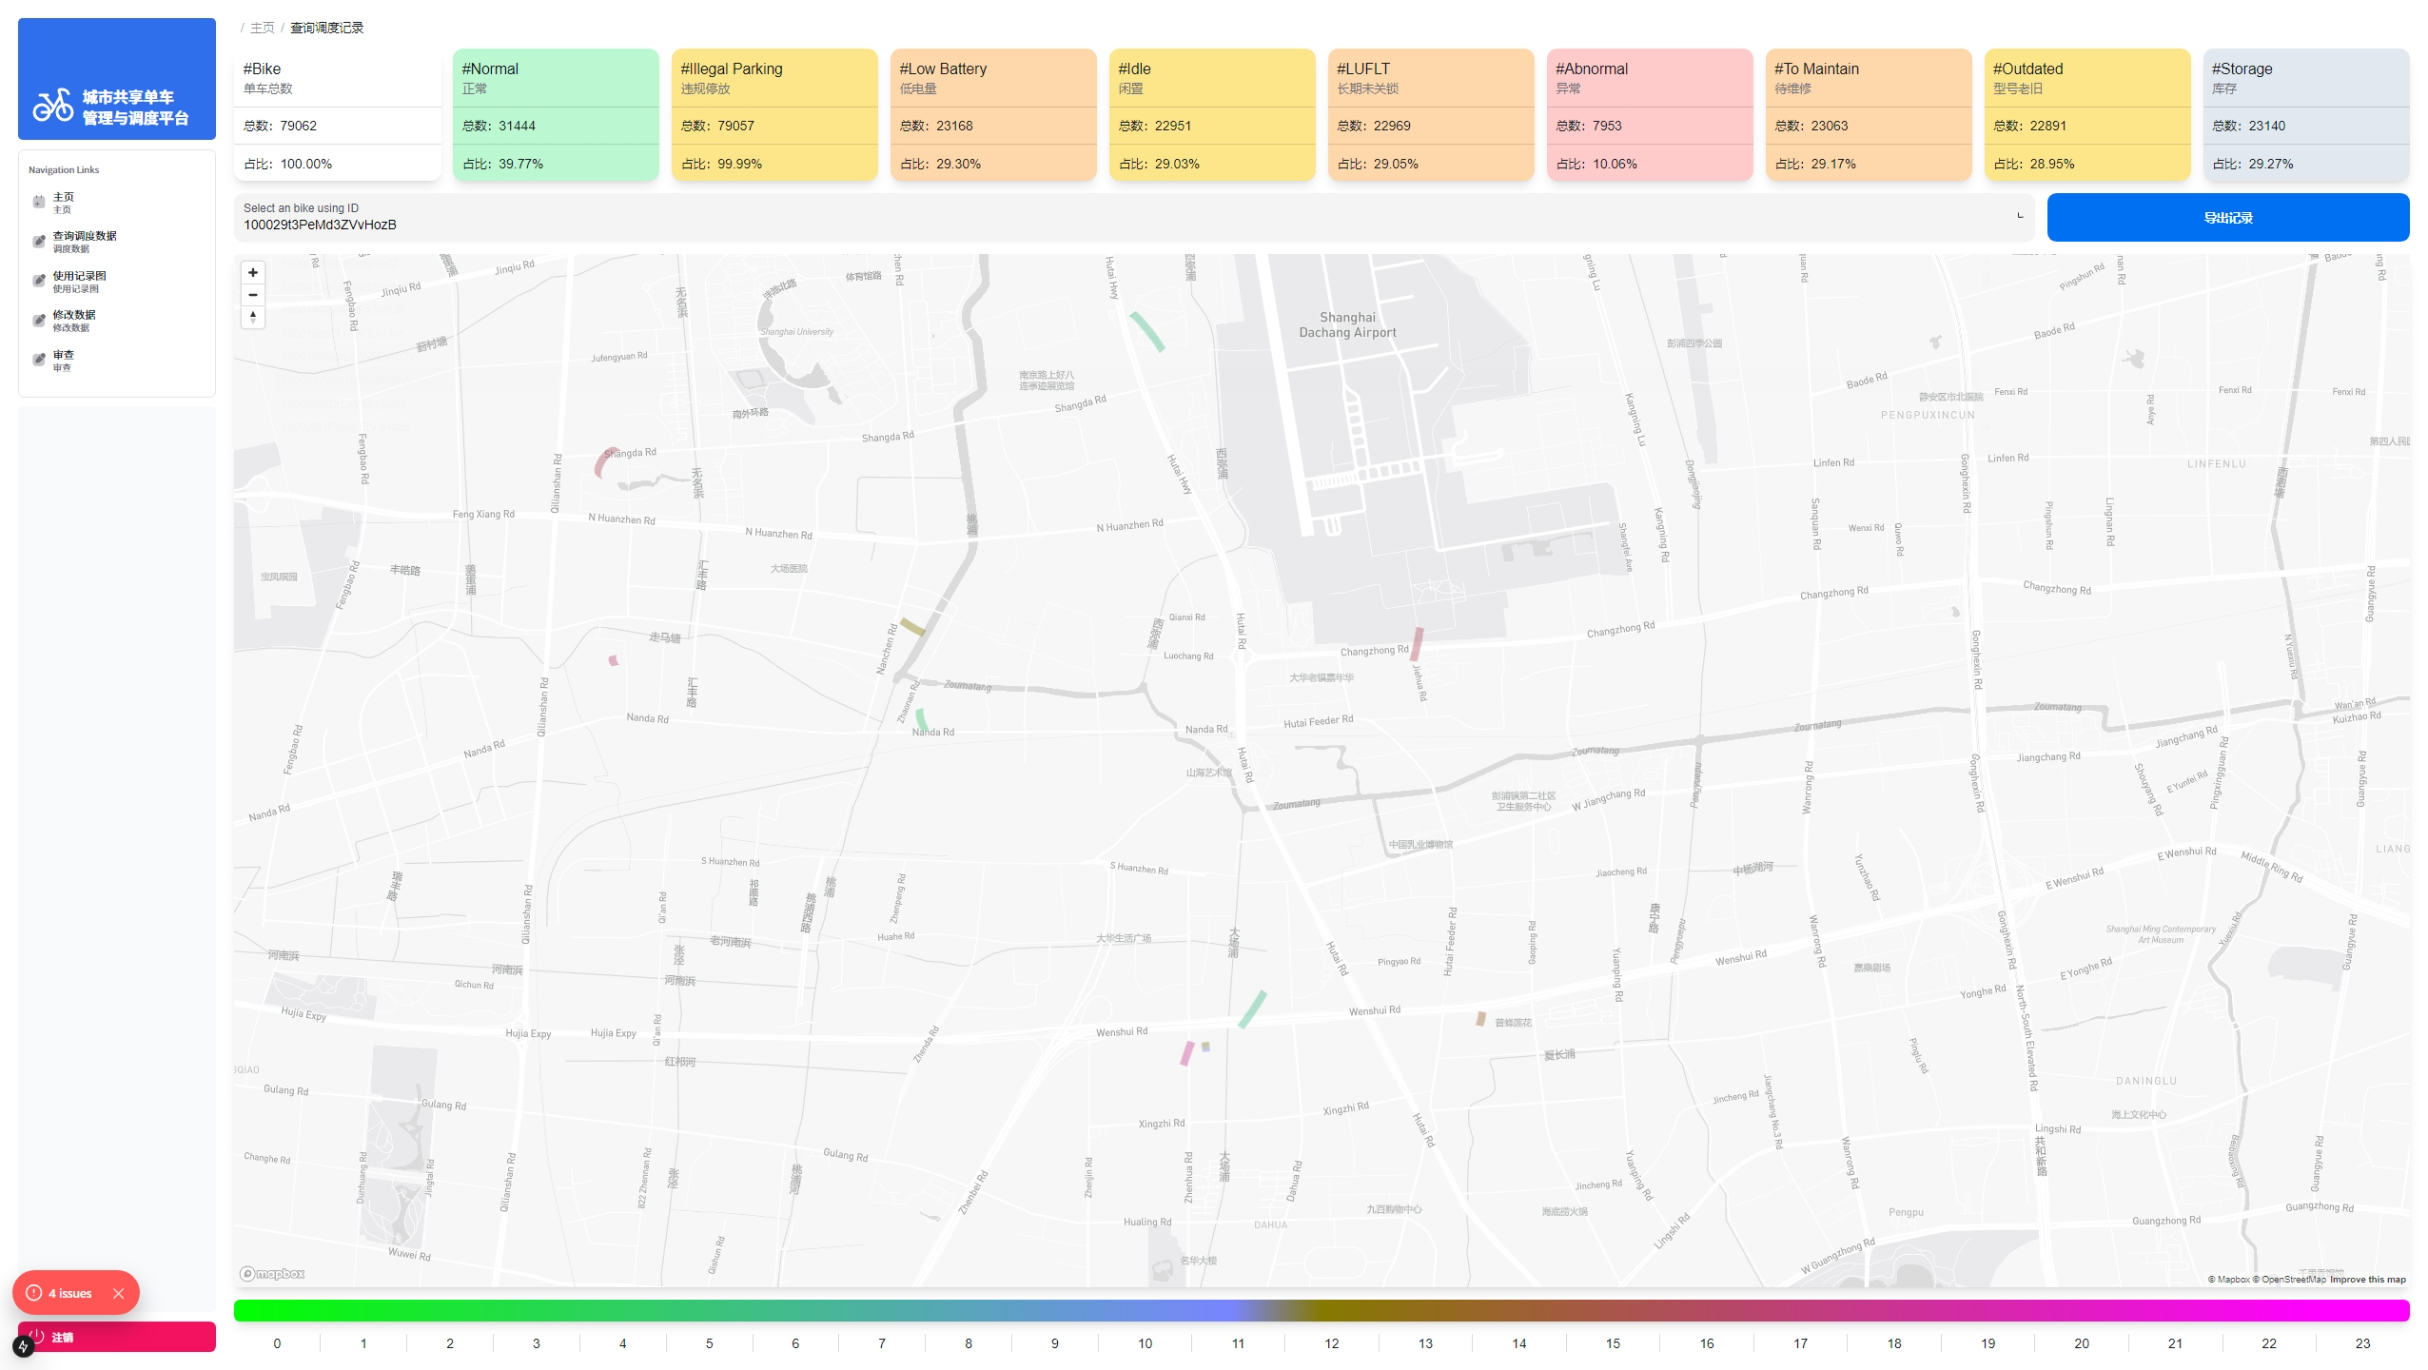
\includegraphics[width=\textwidth]{figures/schedule.png}
    \caption{单车调度记录图}\label{schedule}
\end{figure}

\begin{figure}[!htbp]
    \centering
    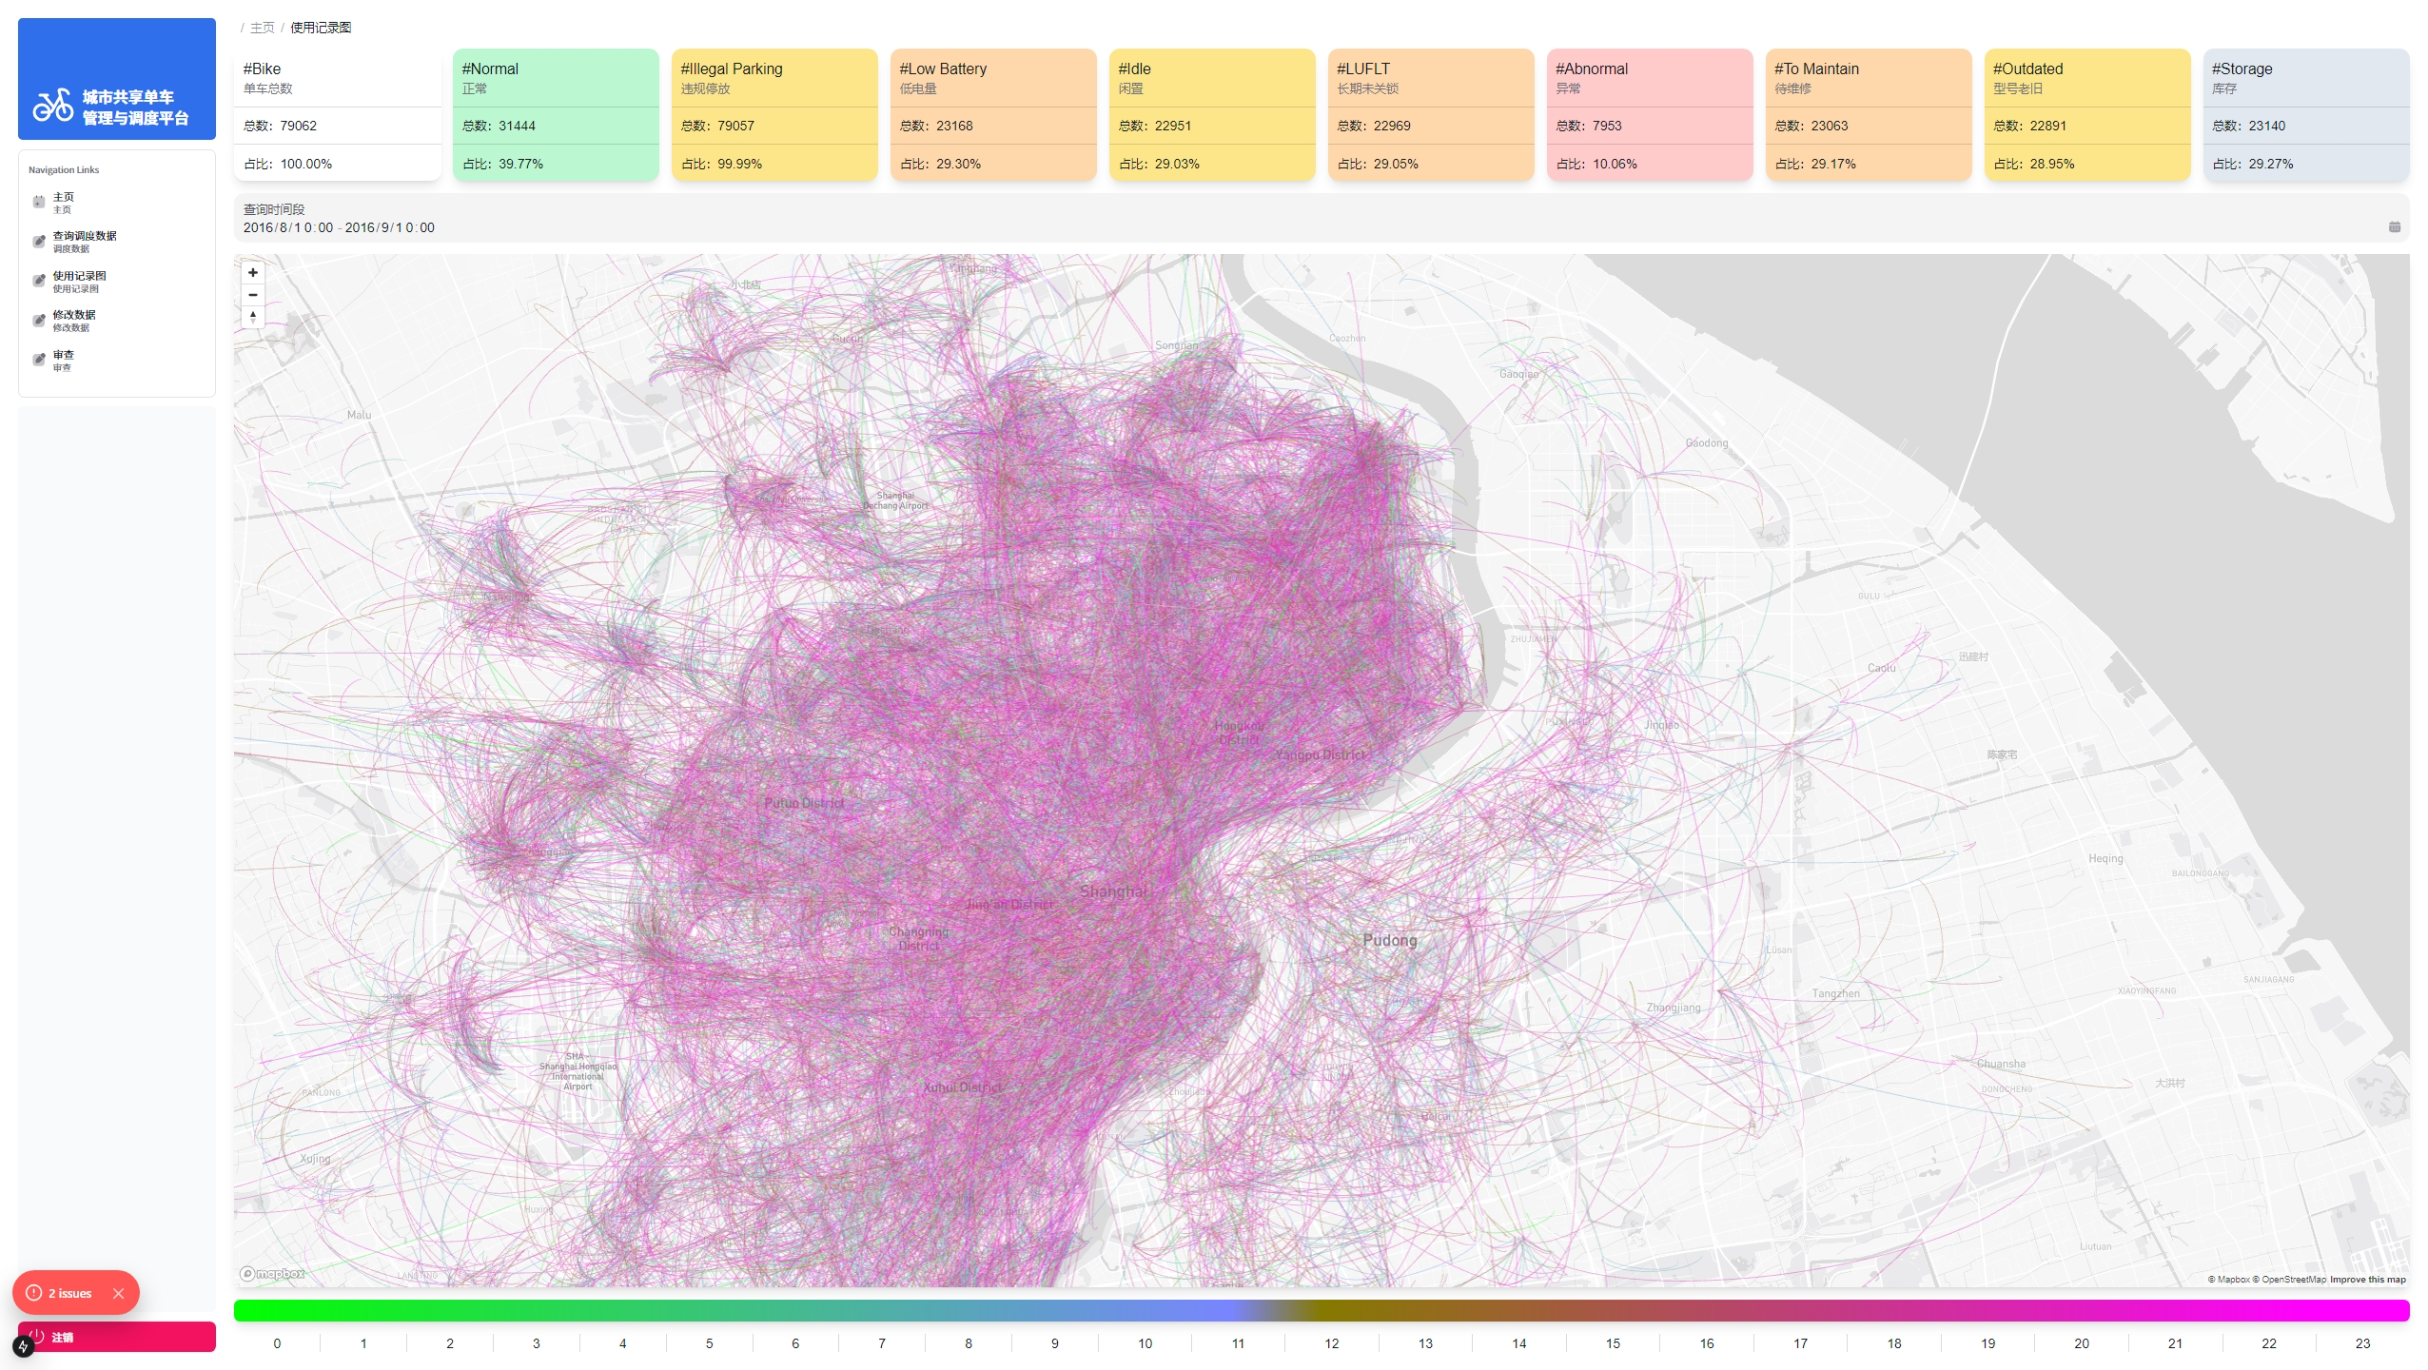
\includegraphics[width=\textwidth]{figures/usage.png}
    \caption{单车使用图}\label{usagePage}
\end{figure}

\begin{figure}[!htbp]
    \centering
    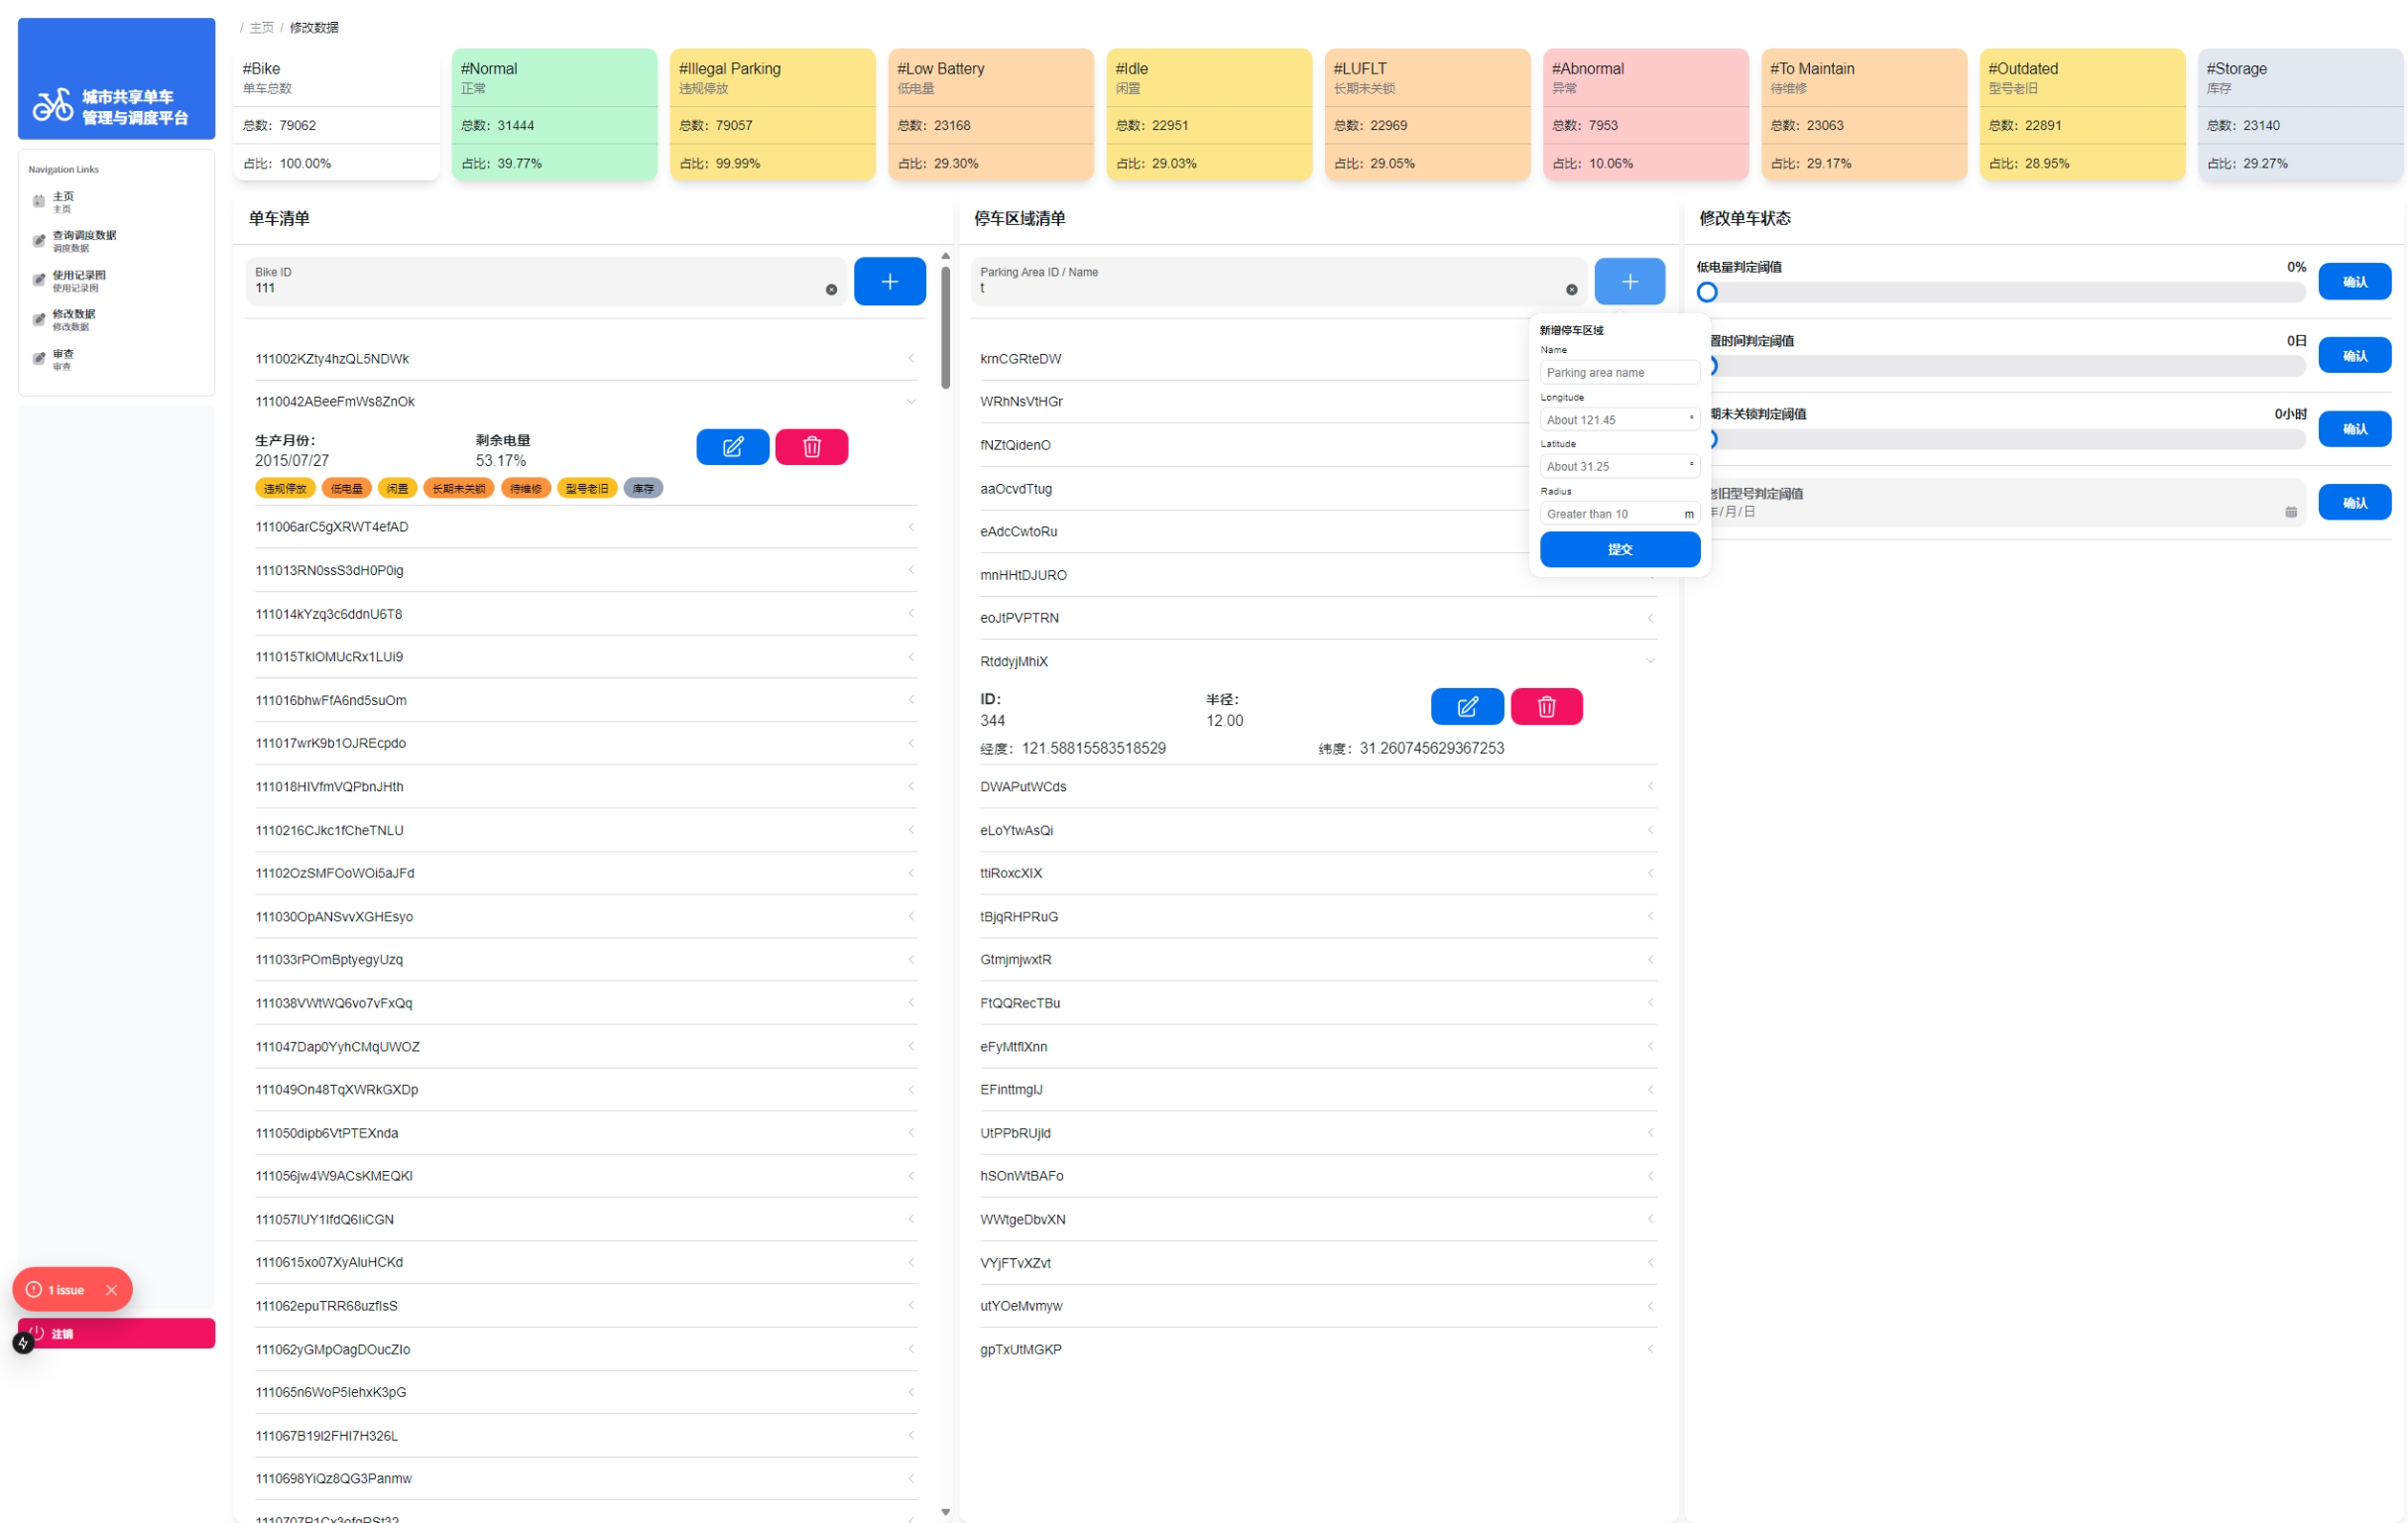
\includegraphics[width=\textwidth]{figures/modify.png}
    \caption{修改页面}\label{modify}
\end{figure}

\begin{figure}[!htbp]
    \centering
    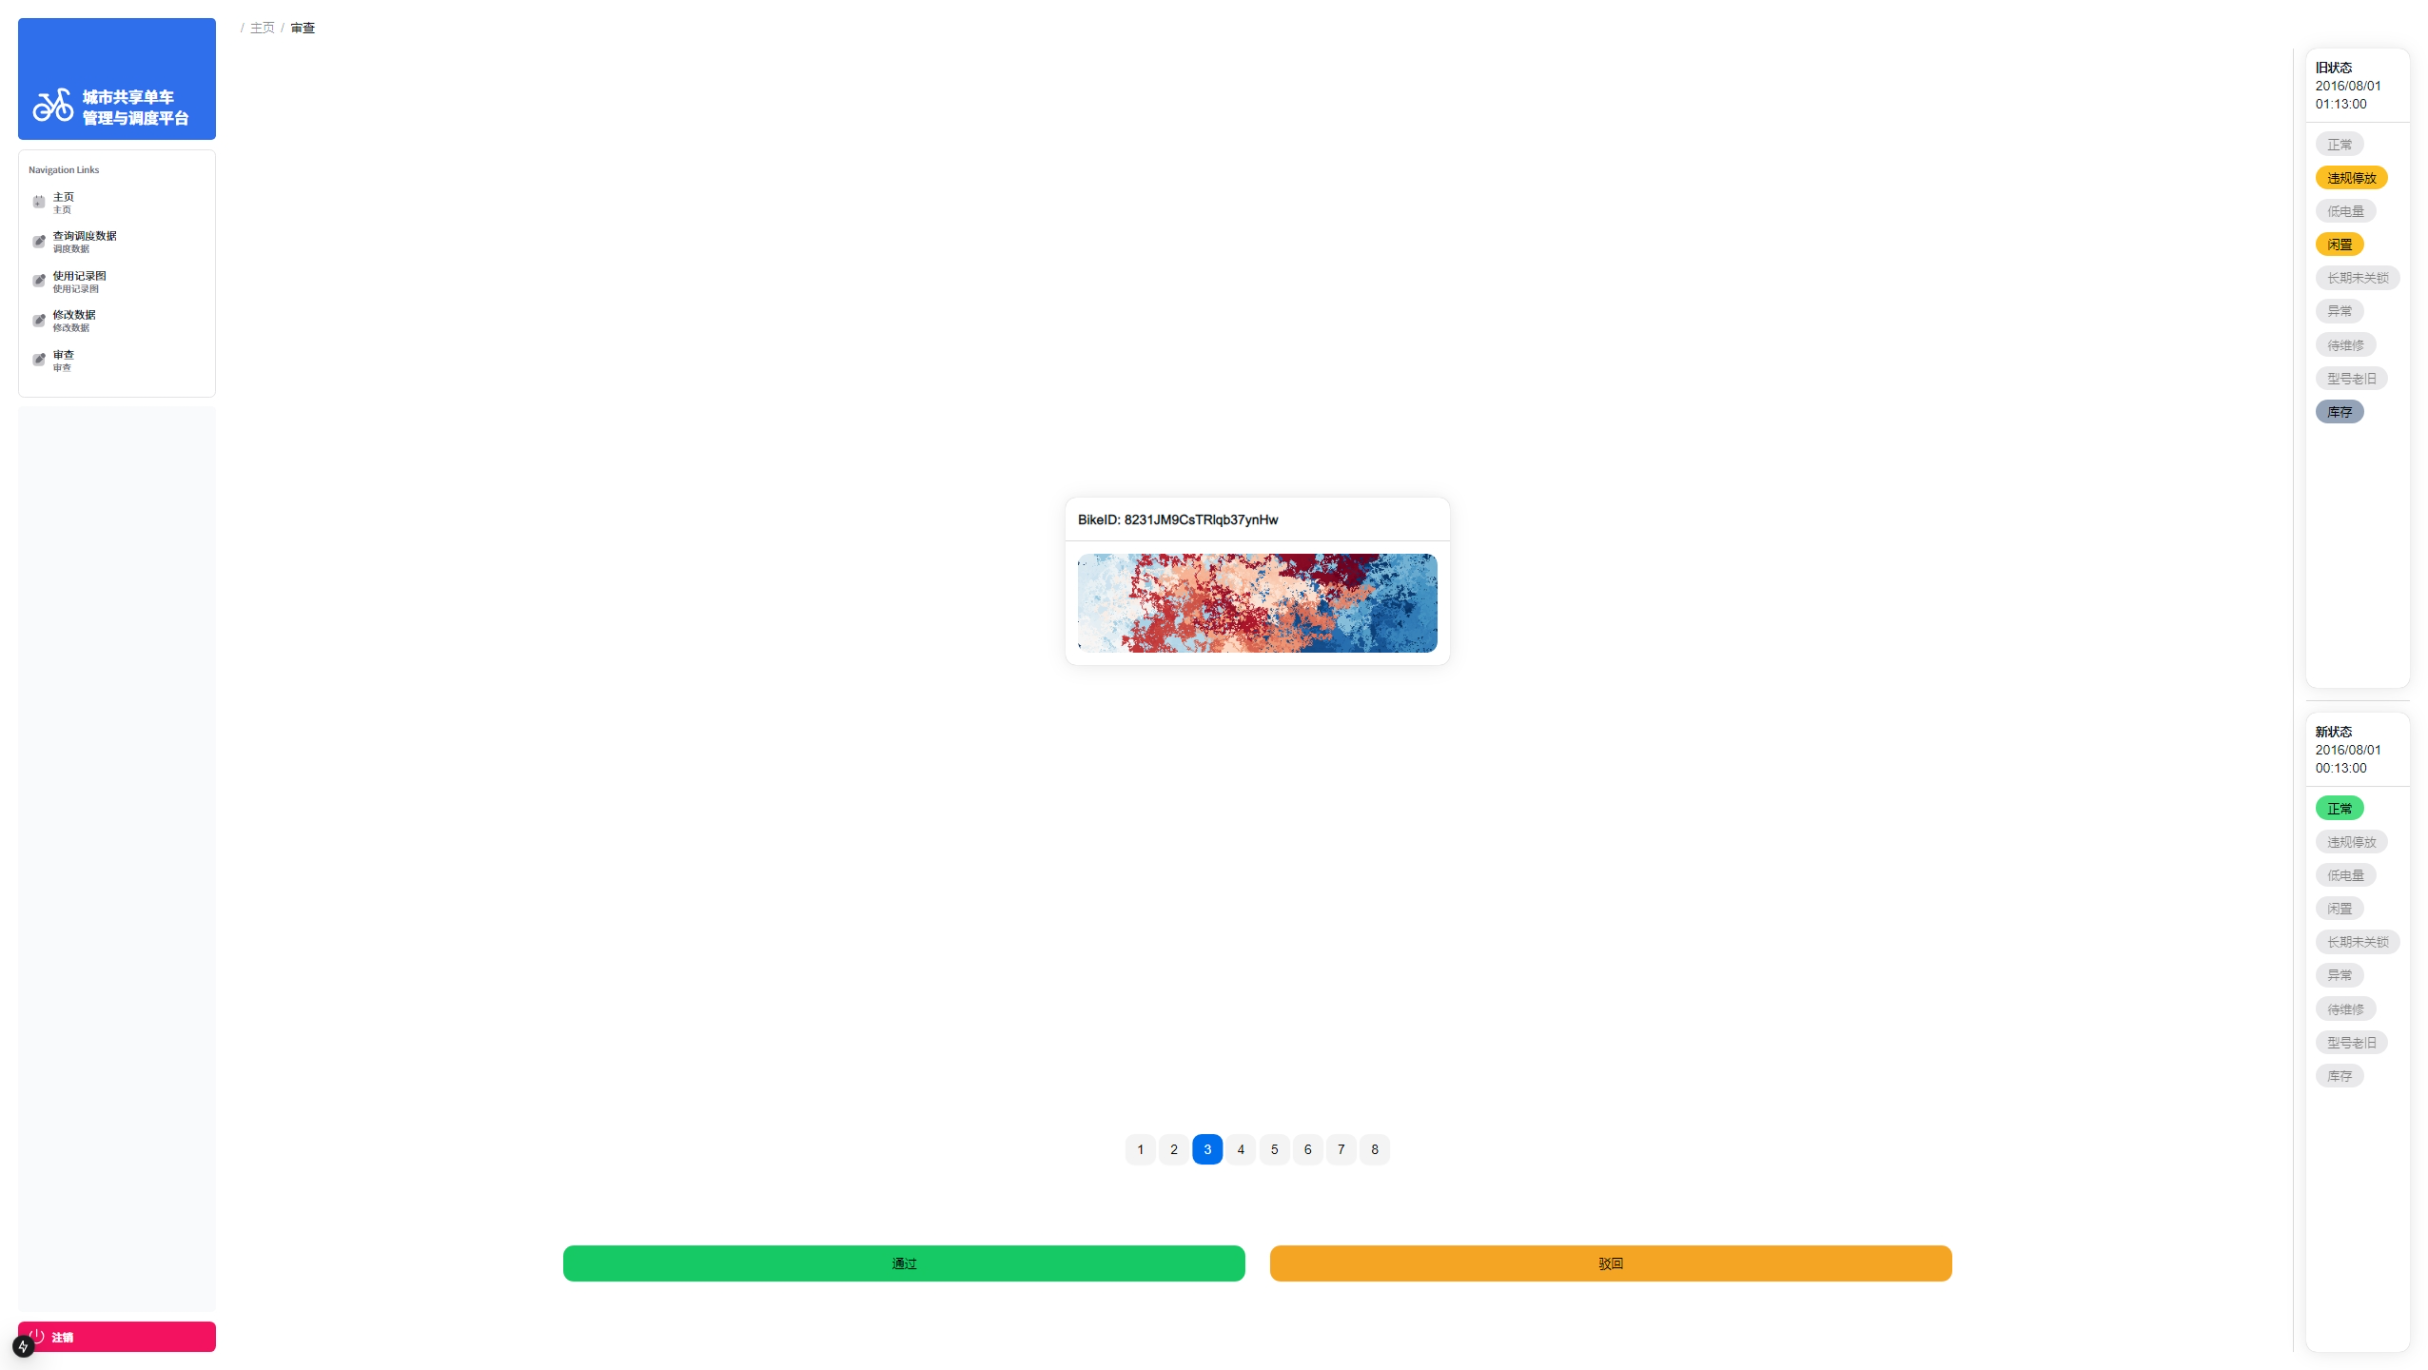
\includegraphics[width=\textwidth]{figures/review.png}
    \caption{审查页面}\label{reviewPage}
\end{figure}

\chapter{总结}
\thispagestyle{empty}
\section{心得体会}
通过本次项目,我收获颇丰。

其一,我通过数据库的设计过程进一步加深了对于上一学期中所学理论知识的理解。

其二,我对于数据库在实际开发过程中的使用有了较为全面的了解。我在本项目中,通过多种方式来和数据交互:
在使用数据来填充数据库的过程中,我使用Python语言来与数据库进行交互;在应用开发过程中,我使用DataGrip和pgAdmin4来对于
数据库进行管理;在应用开发阶段,我是用Drizzle ORM来进行数据的CRUD操作。同时,本项目所使用的数据库涉及到
多种数据类型,例如\textbf{ENUM},\textbf{TEXT},\textbf{point},被用来存储单车状态,图片和坐标等信息;本项目还利用
数据库提供的\verb|crypt|函数来实现对于用户密码的加密存储、利用\textbf{check}约束和触发器来确保数据的一致性;本项目
还利用数据库中的用户定义函数来实现添加用户功能。

其三,通过本次项目我也掌握了开发网页的基本流程的技术栈。对于前端,我学习了React和Tailwind CSS的基本使用方法;
对于后端,我了解了ORM技术、鉴权技术以及Typescript语言的基本使用。同时,我还对于App路由版本的Next.js有了初步了解,
能够利用它来快速开发出一个中小型网页应用。
% \maketitle
% \thispagestyle{fancy}%用于单独设置某页的样式,此处用于设置标题页的格式
\bibliographystyle{IEEEtran}
\bibliography{bib/ref}
\end{document}